\chapter{Sistema/Modelo/Método}

\section{Modelo}
El cubo de Rubik $3 \times 3 \times 3$ está compuesto de $3$ tipos de piezas distintas:
\begin{itemize}
	\item \textbf{Centros}: piezas con un sólo color, que sólo rotan sobre su eje, $6$ en total.
	\item \textbf{Aristas}: piezas con $2$ colores, $12$ en total.
	\item \textbf{Esquinas}: piezas con $3$ colores, $8$ en total.
\end{itemize}
La cantidad total de facelets es entonces $1\times 6 + 2\times 12 + 3\times 8 = 54$.
\begin{figure}[h!]
	\centering
	\subcaptionbox{Centros}{%
		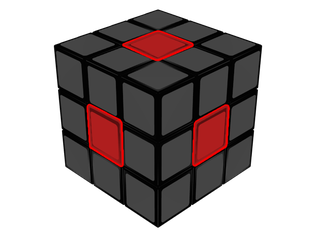
\includegraphics[width=0.30\textwidth]{figures/centers}
	}%
	\hfill
	\subcaptionbox{Aristas}{%
		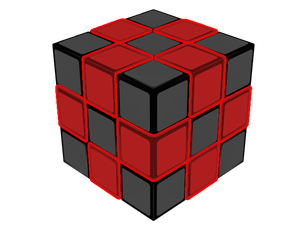
\includegraphics[width=0.30\textwidth]{figures/edges}
	}%
	\hfill
	\subcaptionbox{Esquinas}{%
		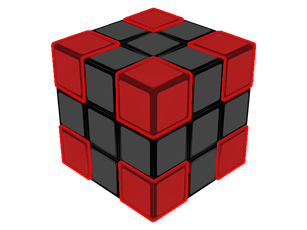
\includegraphics[width=0.30\textwidth]{figures/corners}
	}%
	\caption{Los $3$ tipos de piezas del cubo de Rubik.}
\end{figure}

\subsection{Convenciones}\label{convenciones}
Existe una notación estándar para describir los ejes, las caras y los facelets del cubo~\cite{notationsingmaster}.
Los $3$ ejes de coordenadas del sistema de referencia utilizado se definen de la siguiente manera:
\begin{itemize}
	\item $x$: eje que atraviesa las caras derecha e izquierda del cubo, con respecto al observador.
	\item $y$: eje que atraviesa las caras superior e inferior del cubo.
	\item $z$: eje que atraviesa las caras frontal y trasera del cubo.
\end{itemize}
Así, cada una de las piezas esquina del cubo tiene $1$ color por eje, mientras que las aristas tienen un color en sólo $2$ de los $3$ ejes y los centros en solamente $1$.

Las caras del cubo se identifican mediante la letra inicial de la palabra en inglés que identifica su posición con respecto al observador.
Estas letras son \textbf{U} (up), \textbf{R} (right), \textbf{F} (front), \textbf{D} (down), \textbf{L} (left) y \textbf{B} (bottom).

\begin{figure}[h!]
	\centering
	\subcaptionbox{Ejes}{%
		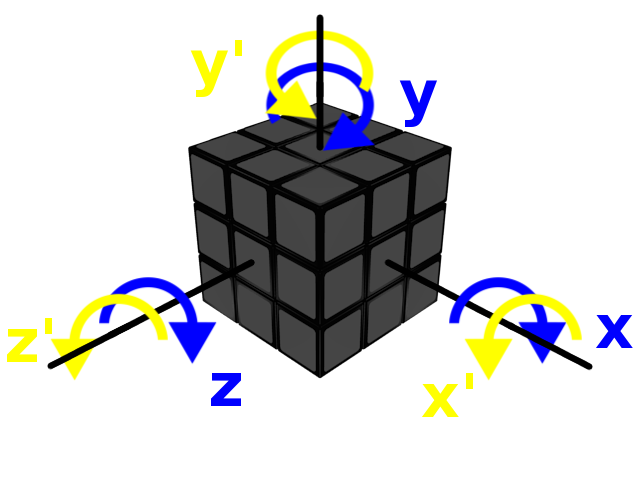
\includegraphics[width=0.45\textwidth]{figures/axes}
	}%
	\hfill
	\subcaptionbox{Caras}{%
		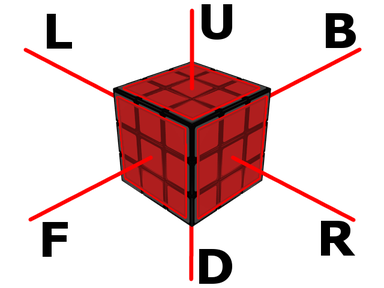
\includegraphics[width=0.45\textwidth]{figures/faces}
	}%
	\caption{Notación de ejes y caras del cubo.}
\end{figure}
De manera similar, los movimientos posibles de cada cara del cubo también quedan descritos por la letra correspondiente de la cara rotada.
En este punto, se decidió adoptar una notación ligeramente diferente de la estándar.
En la notación propuesta, \textit{XN} indica que la cara \textit{X} rota en $90 \times N$ grados, donde los grados se miden en sentido horario con respecto a un vector normal a la superficie de la cara a rotar.
Entonces, por ejemplo ``R$1$'' significa rotar la cara derecha en $90$ (o equivalentemente, $-270$) grados, ``R$2$'' es rotar la cara derecha en $180$ (o $-180$) grados y ``R$3$'' rotar la cara derecha en $270$ (o $-90$) grados.
La razón del por qué usar esta notación es tan sólo un detalle de implementación, pues de esta manera el string que representa cada rotación tiene un largo fijo.

\begin{figure}[h!]
	\centering
	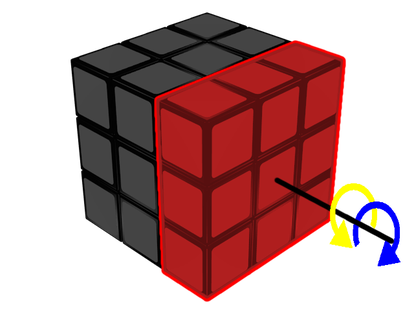
\includegraphics[scale=0.3]{figures/R1}
	\caption[Ejemplo de rotación.]{Flecha azul: movimiento \textit{R1} ($90$ grados sentido horario). Flecha amarilla: movimiento \textit{R3} (90 grados sentido antihorario).}
	\label{moveR}
\end{figure}

Estos ángulos bastan para describir todos los movimientos posibles, ya que $360$ equivale a una operación nula y cualquier otro ángulo dejaría el cubo en un estado inválido, impidiendo los movimientos de algunas de las otras caras.

Las piezas se identifican con las letras de las caras a las que pertenecen. Por lo tanto los centros son \textit{U}, \textit{R}, \textit{F}, \textit{D}, \textit{L} y \textit{B}, las aristas son \textit{UF}, \textit{UR}, \textit{UL}, \textit{UB}, \textit{DF}, \textit{DR}, \textit{DL}, \textit{DB}, \textit{FR}, \textit{FL}, \textit{BR} y \textit{BL} y las esquinas son \textit{URF}, \textit{URB}, \textit{ULF}, \textit{ULB}, \textit{DRF}, \textit{DRB}, \textit{DLF}, y \textit{DLB}.

El estado final del cubo se representó como un arreglo de $54$ elementos, donde cada elemento representa un facelet. El orden de los facelets se muestra en la figura~\ref{faceletorder}.
La asignación de colores a cada cara es totalmente arbitraria y no tiene importancia para el sistema desarrollado. Lo importante es que, una vez se decida una asignación, se mantenga hasta el final.

\tikzset{boxu/.style={draw, minimum width=1cm, minimum height=1cm, fill=red, text=white}}
\tikzset{boxr/.style={draw, minimum width=1cm, minimum height=1cm, fill=blue, text=white}}
\tikzset{boxf/.style={draw, minimum width=1cm, minimum height=1cm, fill=yellow}}
\tikzset{boxd/.style={draw, minimum width=1cm, minimum height=1cm, fill=orange, text=white}}
\tikzset{boxl/.style={draw, minimum width=1cm, minimum height=1cm, fill=red, text=white}}
\tikzset{boxl/.style={draw, minimum width=1cm, minimum height=1cm, fill=green}}
\tikzset{boxb/.style={draw, minimum width=1cm, minimum height=1cm, fill=white}}
\tikzset{boxx/.style={draw, minimum width=1cm, minimum height=1cm, fill=red, text=white}}
\tikzset{boxy/.style={draw, minimum width=1cm, minimum height=1cm, fill=green}}
\tikzset{boxz/.style={draw, minimum width=1cm, minimum height=1cm, fill=blue, text=white}}
\tikzset{boxc/.style={draw, minimum width=1cm, minimum height=1cm}}

\begin{figure}[h!]
	\centering
	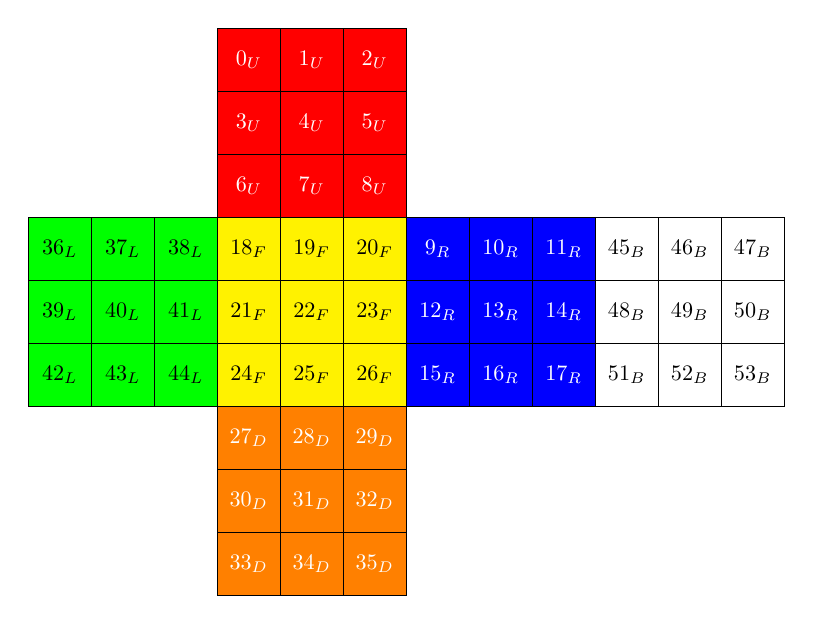
\begin{tikzpicture}[scale=0.8,every node/.style={scale=0.8}]
		\foreach \x in {0,...,2} {
			\foreach \y in {0,...,2} {
			 	\pgfmathsetmacro\result{int(3*\x+\y)}
				\node[boxu] at (3+\y, 8-\x) {$\result_U$};
			}
		}
		\foreach \x in {0,...,2} {
			\foreach \y in {0,...,2} {
				\pgfmathsetmacro\result{int(3*\x+\y + 36)}
				\node[boxl] at (\y, 5-\x) {$\result_L$};
			}
		}
		\foreach \x in {0,...,2} {
			\foreach \y in {0,...,2} {
				\pgfmathsetmacro\result{int(3*\x+\y + 18)}
				\node[boxf] at (\y+3, 5-\x) {$\result_F$};
			}
		}
		\foreach \x in {0,...,2} {
			\foreach \y in {0,...,2} {
				\pgfmathsetmacro\result{int(3*\x+\y + 9)}
				\node[boxr] at (\y+6, 5-\x) {$\result_R$};
			}
		}
		\foreach \x in {0,...,2} {
			\foreach \y in {0,...,2} {
				\pgfmathsetmacro\result{int(3*\x+\y + 45)}
				\node[boxb] at (\y+9, 5-\x) {$\result_B$};
			}
		}
		\foreach \x in {0,...,2} {
			\foreach \y in {0,...,2} {
				\pgfmathsetmacro\result{int(3*\x+\y + 27)}
				\node[boxd] at (\y+3, 2-\x) {$\result_D$};
			}
		}
	\end{tikzpicture}
	\caption[Orden de los facelets.]{Orden de los facelets. El valor representa su posición el arreglo y el subíndice la cara a la que pertenece.}
	\label{faceletorder}
\end{figure}

\section{Sistema}
El sistema desarrollado consiste de varios módulos que pueden agruparse según su función en las siguientes categorías:
\begin{description}
	\item[Manipulación:] Módulos que se encargan de mover las articulaciones y controlar las pinzas del robot.
	\item[Visión:] Módulos encargados de la detección del estado del cubo.
	\item[Resolución:] Módulo encargado de buscar una secuencia de rotaciones de caras que lleven al cubo a su estado resuelto.
\end{description}

\subsection{Manipulación}
Consiste de los módulos que se encargan de la parte hardware del sistema, es decir los movimientos de las articulaciones del robot y la apertura, cierre y calibración de los grippers. Para mover los brazos del robot se usa una combinación de cinemáticas inversas y manipulación directa de ángulos de sus articulaciones.

Las tareas requeridas incluyen:
\begin{enumerate}
	\item Recoger el cubo.
	\item Acercar el cubo a una cámara para detectar su estado.
	\item Realizar rotaciones de las caras.
	\item Mover el cubo de un brazo a otro cuando sea necesario.
\end{enumerate}

El robot Baxter posee varios tipos de grippers, mostrados en la figura~\ref{grippers}. Por el tamaño del cubo, se utilizó el gripper largo y angosto, para tener un agarre lo suficientemente profundo y firme.

\begin{figure}[h!]
	\centering
	\subcaptionbox{Gripper 1.}{%
		\includegraphics[width=0.24\textwidth]{figures/gripper_a}
	}%
	\hfill
	\subcaptionbox{Gripper 2.}{%
		\includegraphics[width=0.24\textwidth]{figures/gripper_c}
	}%
	\hfill
	\subcaptionbox{Gripper 3.}{%
		\includegraphics[width=0.24\textwidth]{figures/gripper_d}
	}%
	\hfill
	\subcaptionbox{Gripper 4.}{%
		\includegraphics[width=0.24\textwidth]{figures/gripper_b}
	}%
	\caption[Pinzas disponibles.]{Grippers disponibles. Los de la figura (a) sólo permiten rotar una cara sin cambiar de mano el cubo. Los de la figura (b) son más anchos que el largo de las caras del cubo. Los de la figura (c) son muy cortos para tener un agarre estable. Los de la figura (d) fueron los gripper utilizados.}
	\label{grippers}
\end{figure}

Los agarres son siempre de la forma como se muestra en la figura~\ref{agarreadecuado}. Esto impide la rotación de tres caras: las $2$ que tocan los grippers y la cara que está más cercana al brazo del robot. La manera en que se realizan las rotaciones es que un brazo sostiene el cubo en una orientación cómoda para que el otro brazo se acerque y agarre una cara no bloqueada de manera perpendicular, y la gire en $90$, $180$ o $270$ grados según corresponda. Esto permite rotar libremente $3$ caras. Para rotar las otras $3$, \textbf{se cambia el cubo al otro brazo}, para que éste lo sostenga en una forma que libere las caras previamente bloqueadas.

\begin{figure}[h!]
	\centering
	\subcaptionbox{Agarre poco profundo, inestable.}{%
		\includegraphics[width=0.35\textwidth]{figures/small_agarre_corto}
	}%
	\hfill
	\subcaptionbox{Agarre utilizado. $3$ caras libres para rotar. Estable.\label{agarreadecuado}}{%
		\includegraphics[width=0.35\textwidth]{figures/small_agarre_adecuado}
	}%
	\hfill
	\subcaptionbox{Agarre profundo, cara lejana (roja) bloqueada.}{%
		\includegraphics[width=0.35\textwidth]{figures/small_agarre_profundo}
	}%
	\hfill
	\subcaptionbox{Agarre impreciso, cara lateral (marrón) bloqueada. Inestable.}{%
		\includegraphics[width=0.35\textwidth]{figures/small_agarre_desplazado}
	}%
	\caption{Diferentes agarres.}
	\label{agarre}
\end{figure}

\subsubsection{Recogida}
La ejecución comienza con el cubo en la mesa, en una posición marcada cuyas coordenadas son conocidas. Los ejes se definieron con respecto al observador mirando de frente al robot, y no con respecto al punto de vista del robot. Utilizando el servicio de cinemáticas inversas de Baxter, se lleva el brazo izquierdo a una posición cercana al cubo, con las pinzas apuntando hacia abajo, para luego recogerlo. Este agarre bloquea las caras \textit{L}, \textit{R} y \textit{U}.

\begin{figure}[h!]
	\centering
	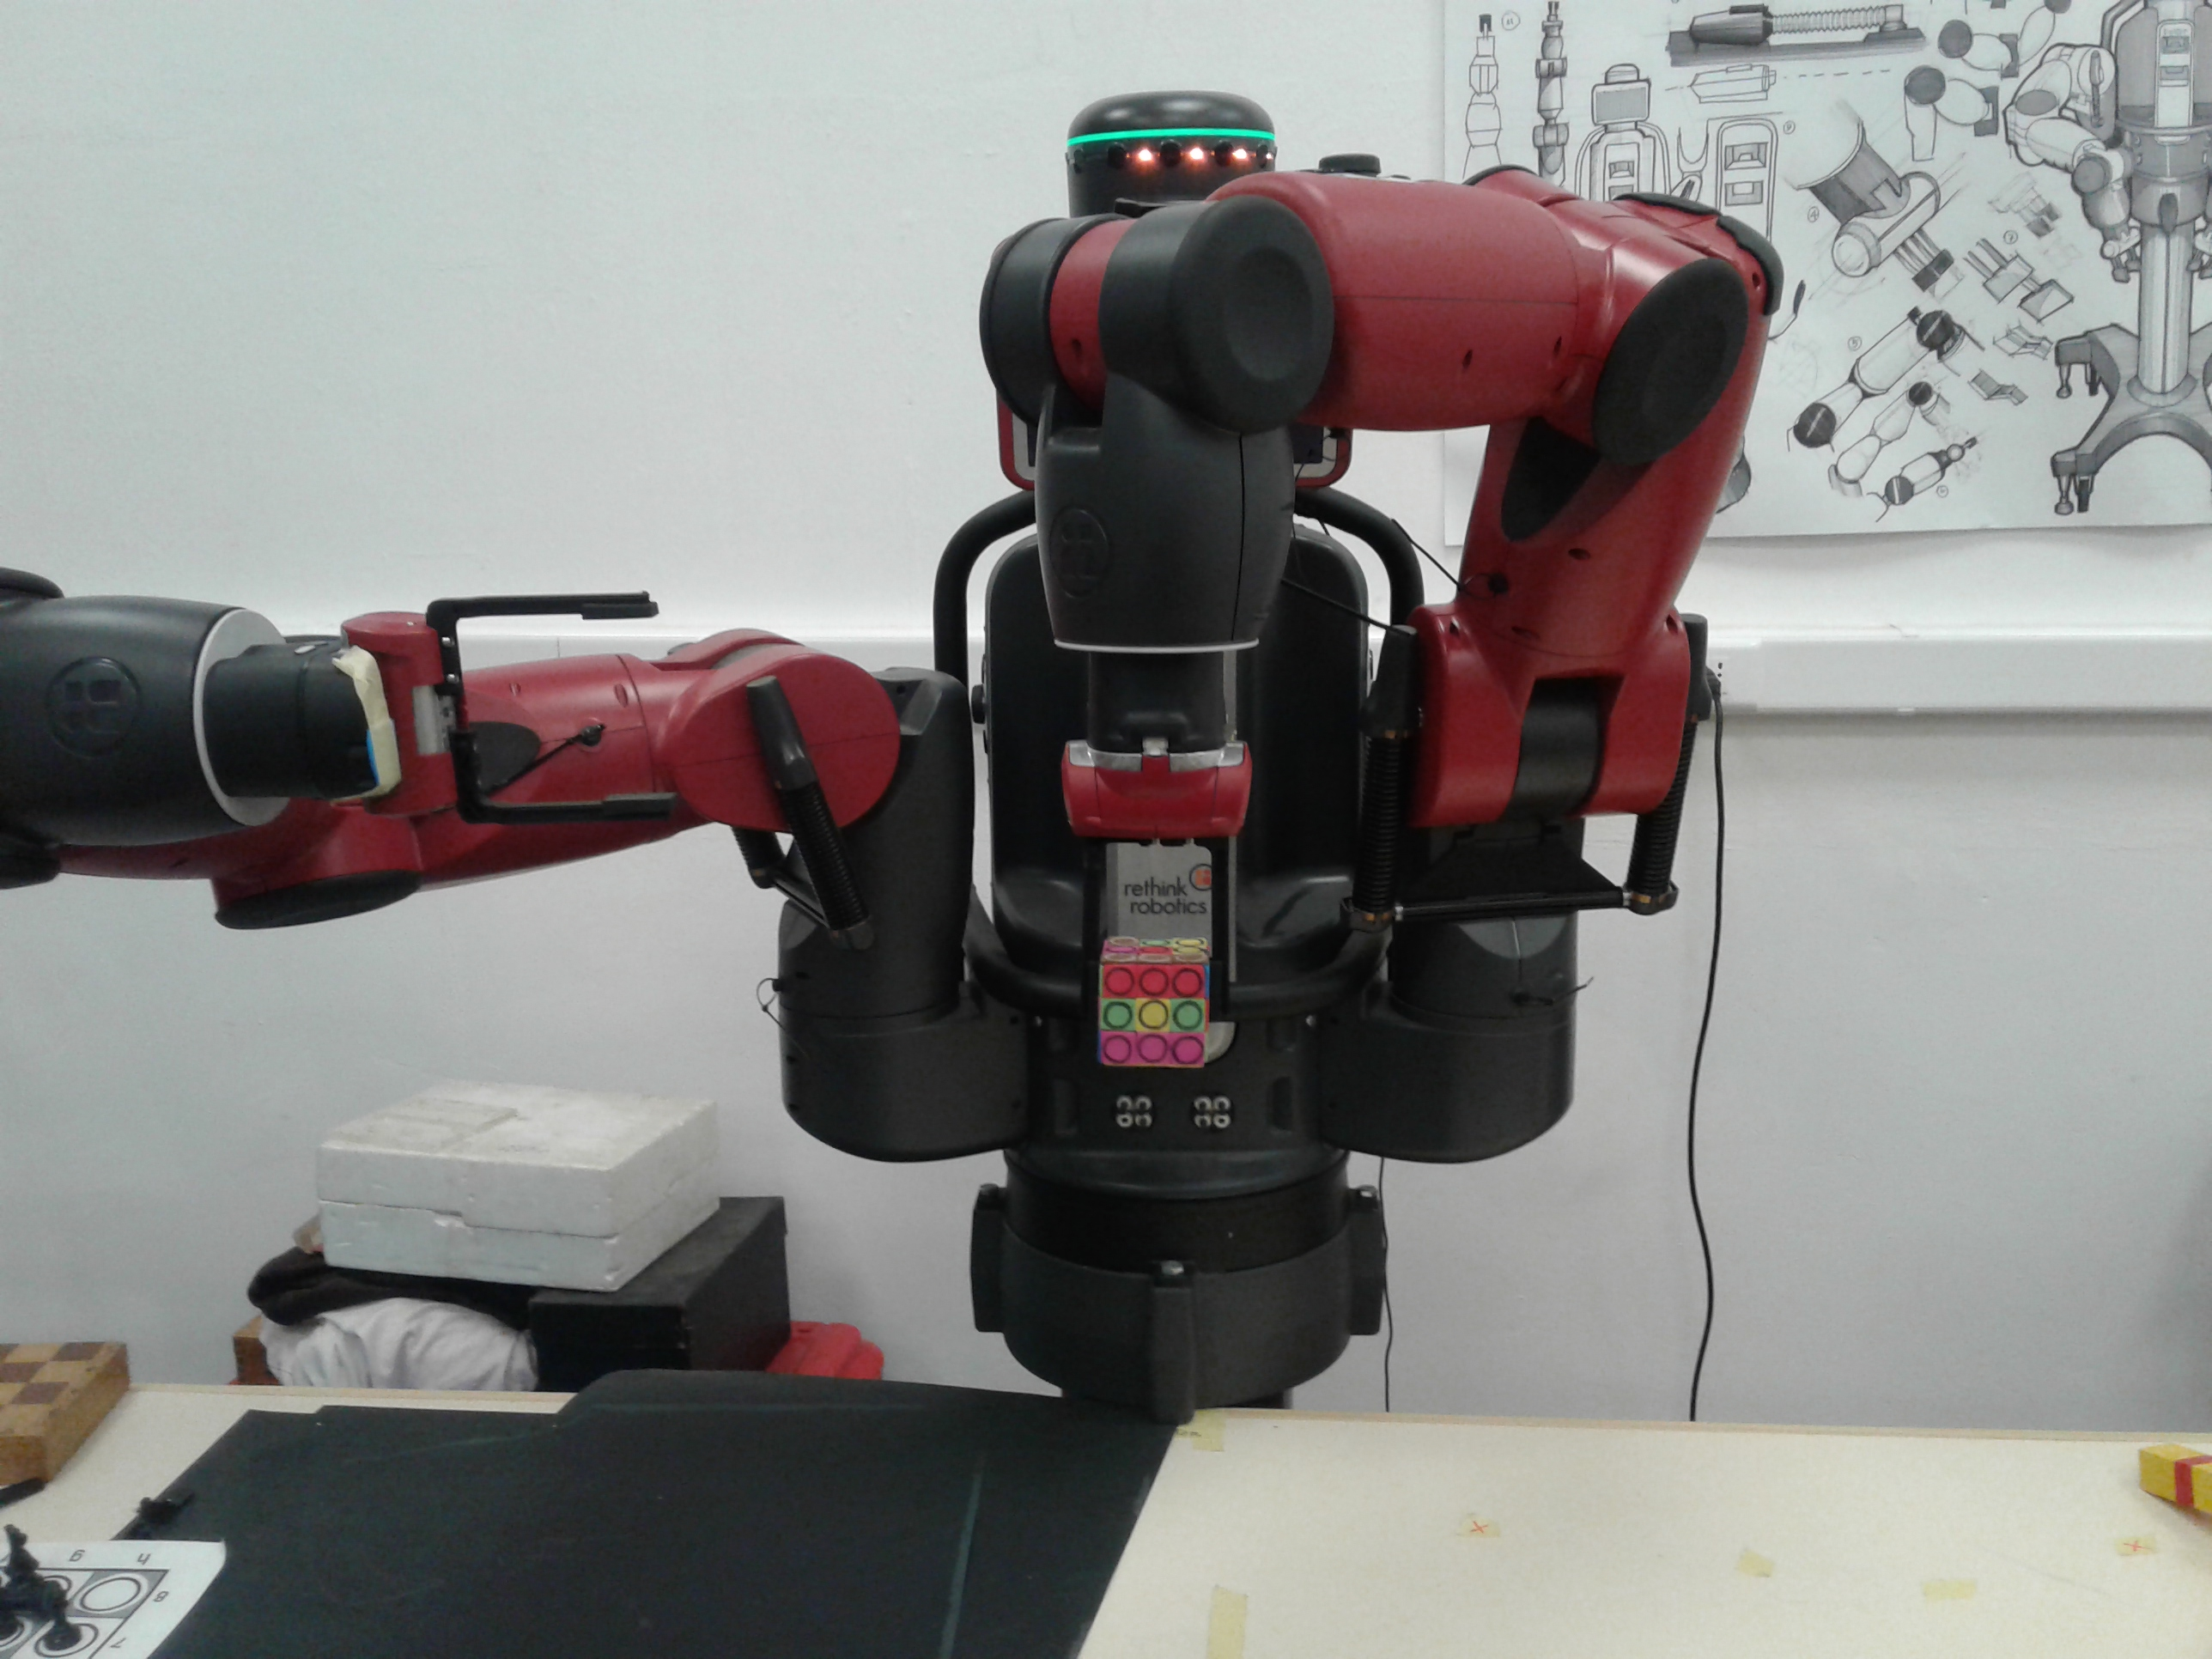
\includegraphics[scale=0.1]{figures/pick}
	\caption[Posición y orientación al recoger el cubo.]{Posición y orientación al recoger el cubo. Los grippers tocan las caras \textit{L} y \textit{R}.}
	\label{pick}
\end{figure}

\subsubsection{Acercamiento a cámara}
El servicio de cinemáticas inversas, si bien garantiza la posición y orientación final solicitada para un gripper, no especifica nada sobre la trayectoria a realizar. Esto puede causar varios problemas, entre ellos los más graves son: la imposibilidad de llevar a cabo un movimiento debido a la complejidad de la trayectoria, a pesar de que sea una configuración válida; y la ejecución de ciertas trayectorias que causan que el robot se golpee a sí mismo. Debido a la naturaleza misma de IK, no es posible predecir cuándo suceden estos errores. Así que en este paso se mueve el brazo utilizando directamente los ángulos de cada una de sus articulaciones, para guiarlo a una configuración favorable, seguido inmediatamente por cinemáticas inversas para obtener la posición y orientación final deseada. Las $6$ configuraciones necesarias para apuntar cada cara a la cámara se muestran en la figuras \ref{caml} y \ref{camr}.

\begin{figure}[h!]
	\centering
	\subcaptionbox{Capturando la cara \textit{F}}{%
		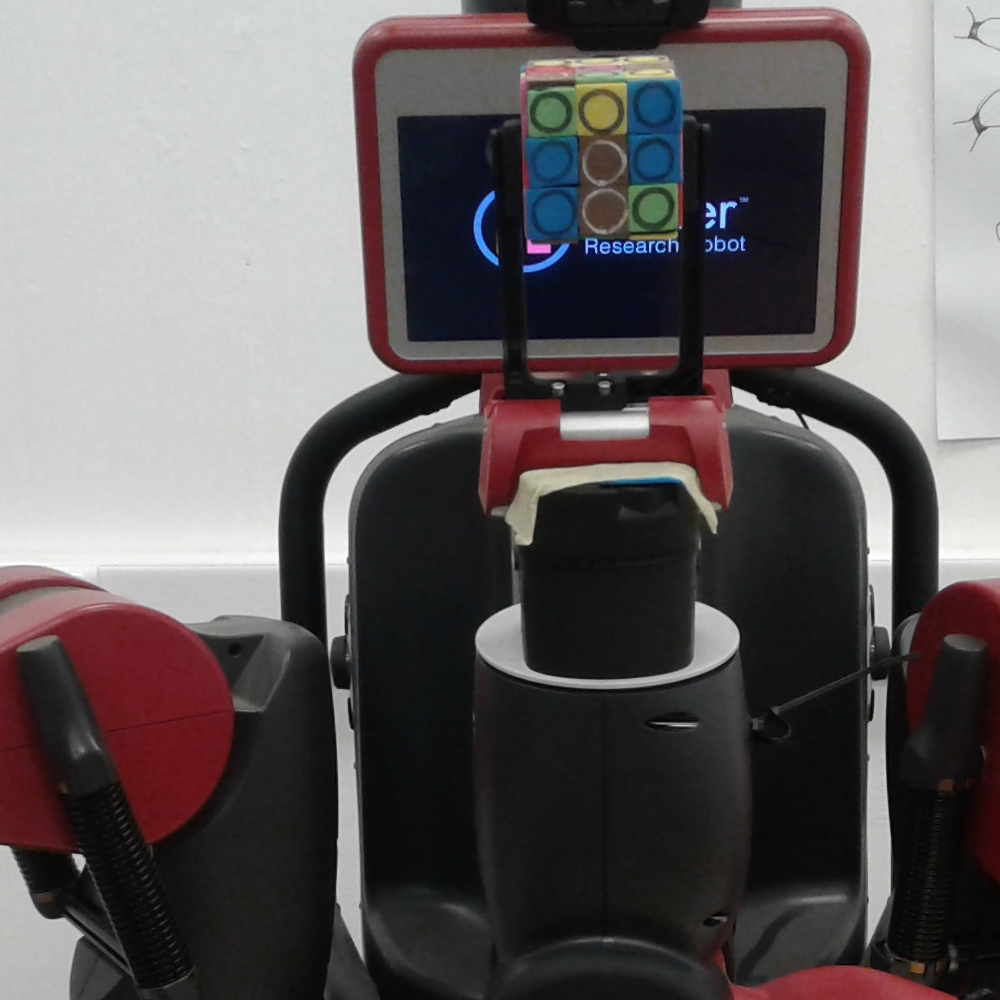
\includegraphics[width=0.30\textwidth]{figures/small_capture_F}
	}%
	\hfill
	\subcaptionbox{Capturando la cara \textit{D}}{%
		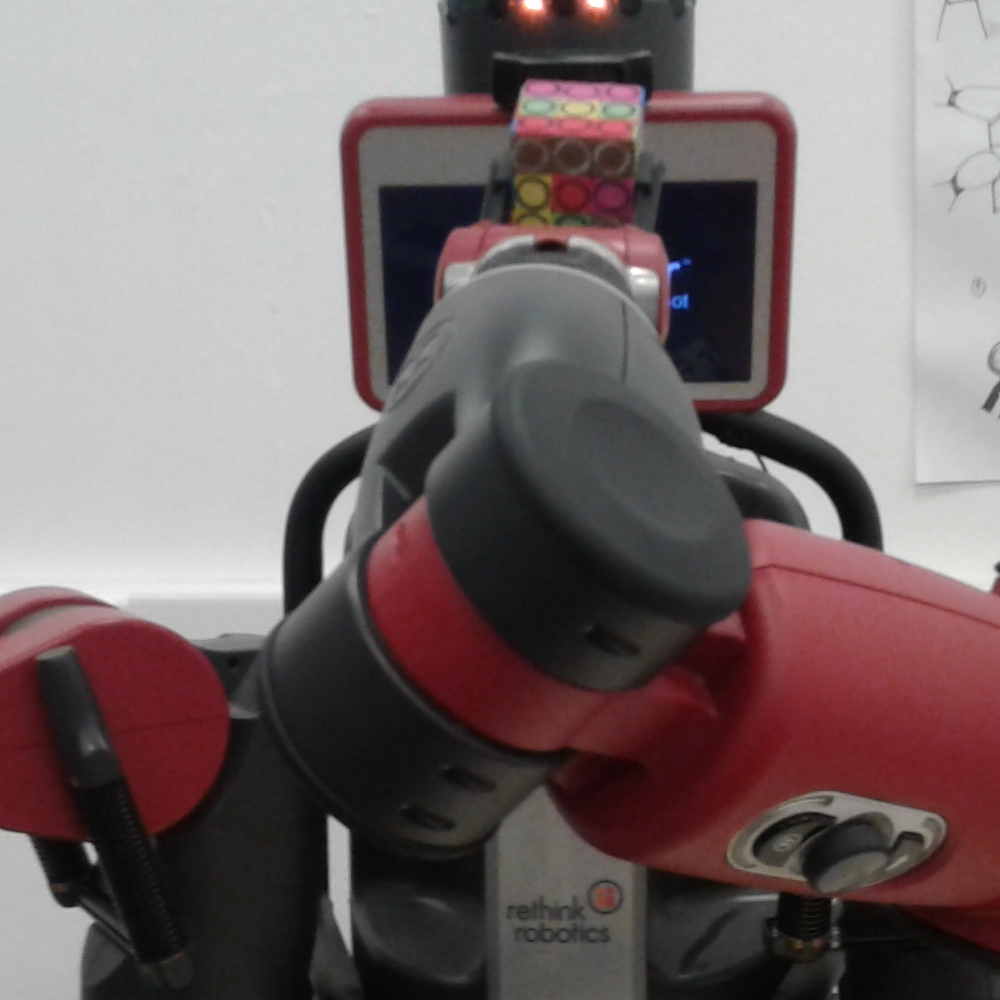
\includegraphics[width=0.30\textwidth]{figures/small_capture_D}
	}%
	\hfill
	\subcaptionbox{Capturando la cara \textit{B}}{%
		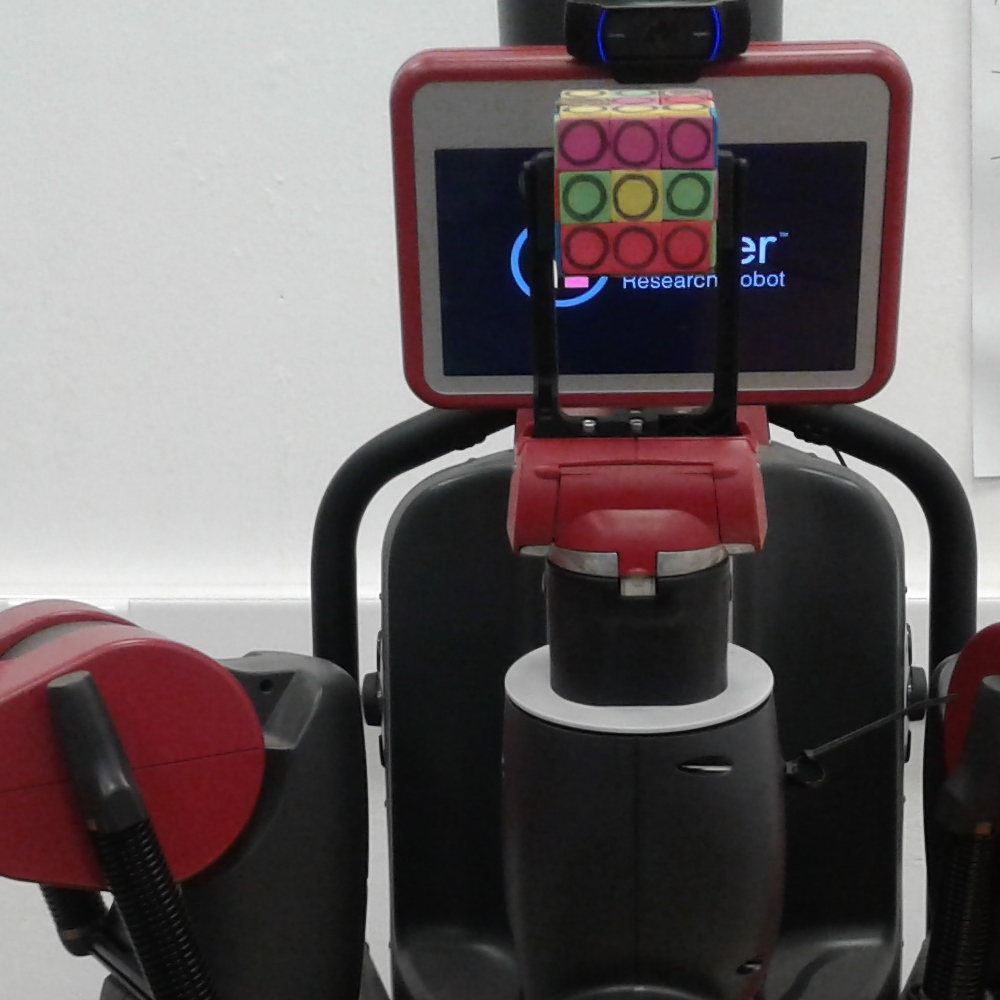
\includegraphics[width=0.30\textwidth]{figures/small_capture_B}
	}%
	\caption{Configuraciones del brazo izquierdo para acercamiento a la cámara.}
	\label{caml}
\end{figure}
\begin{figure}[h!]
	\centering
	\subcaptionbox{Capturando la cara \textit{L}}{%
		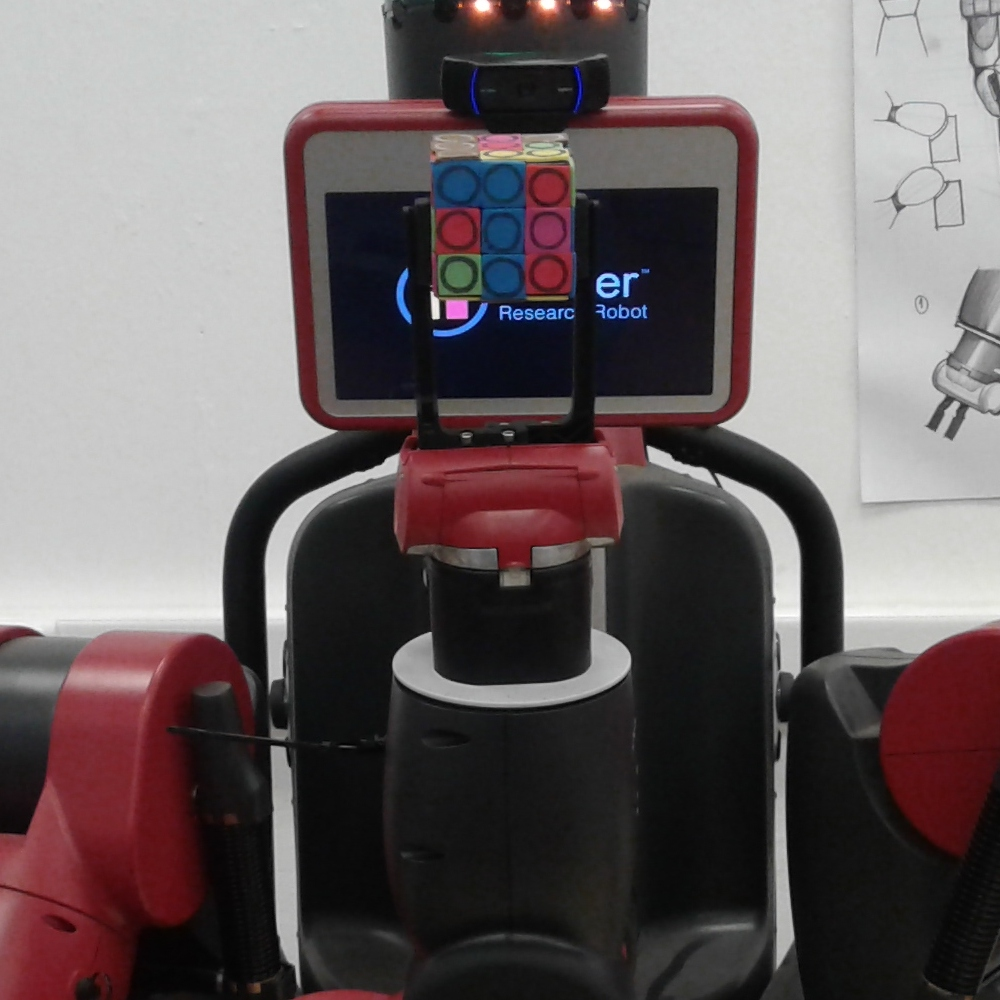
\includegraphics[width=0.30\textwidth]{figures/small_capture_L}
	}%
	\hfill
	\subcaptionbox{Capturando la cara \textit{U}}{%
		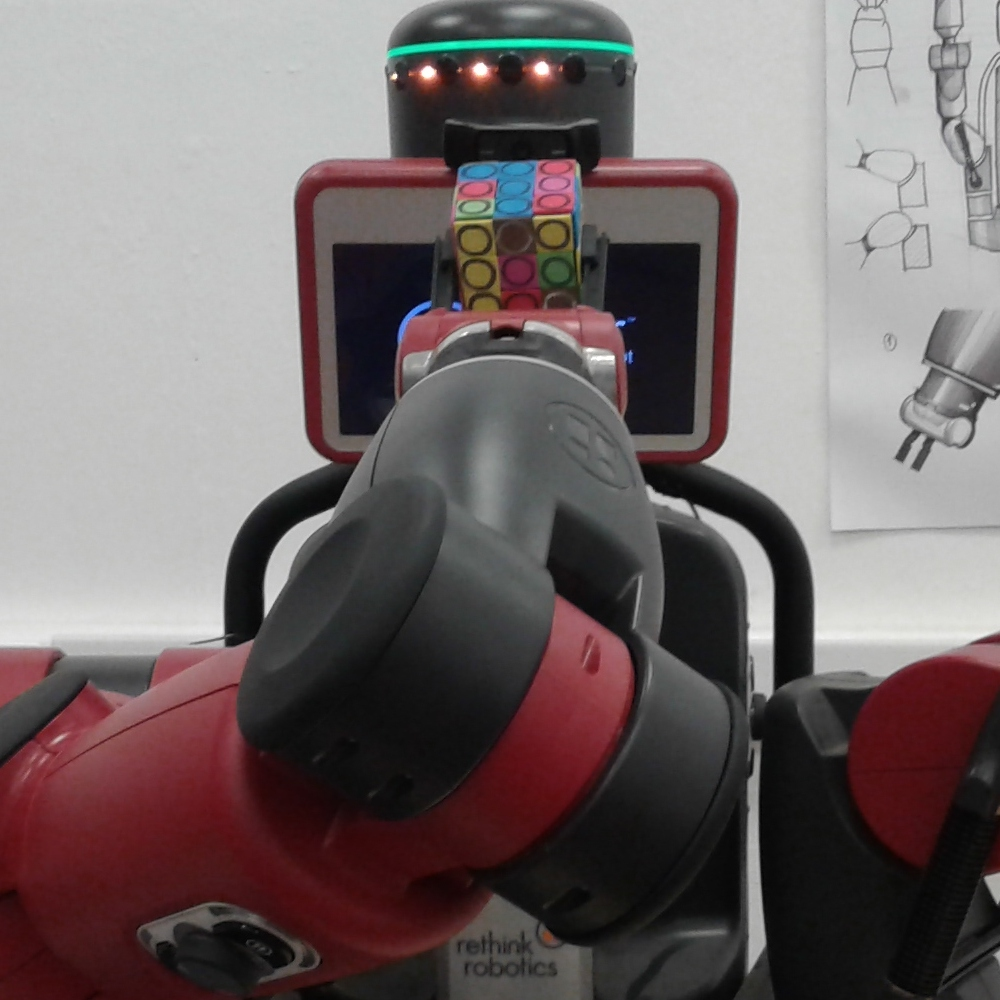
\includegraphics[width=0.30\textwidth]{figures/small_capture_U}
	}%
	\hfill
	\subcaptionbox{Capturando la cara \textit{R}}{%
		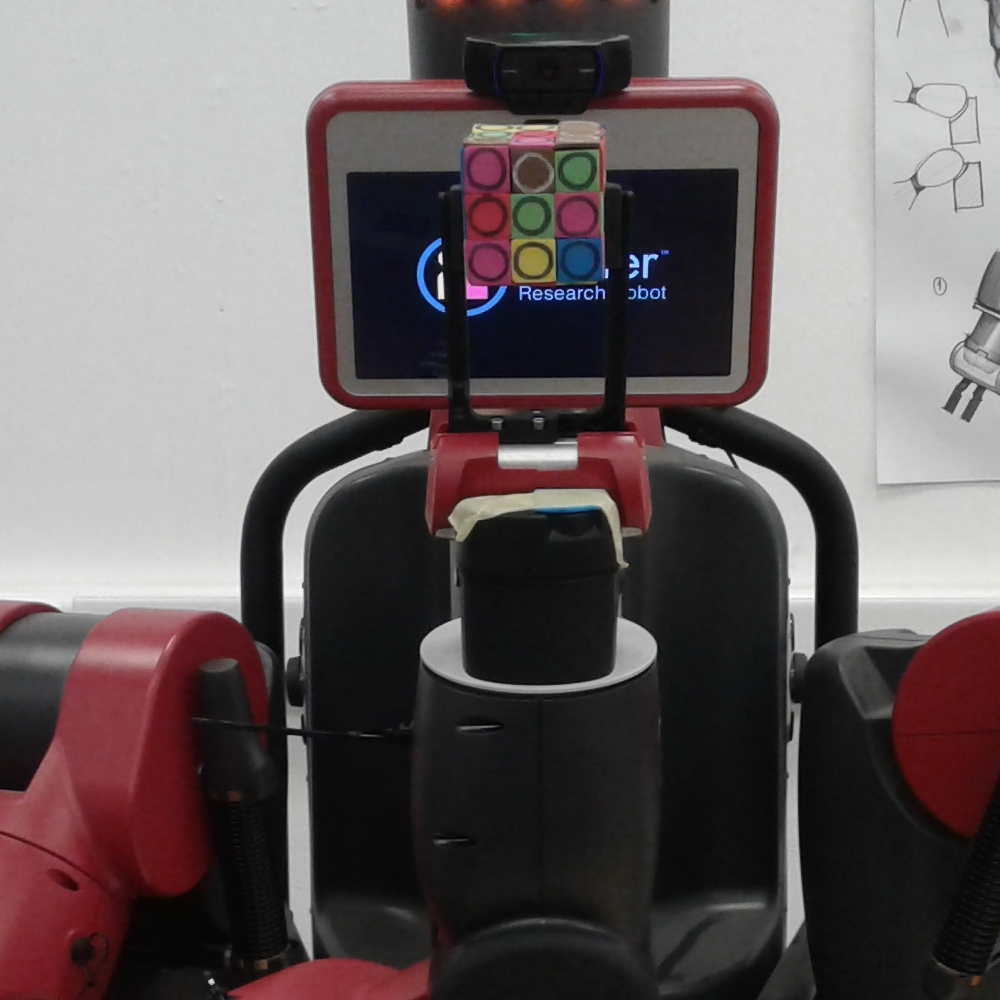
\includegraphics[width=0.30\textwidth]{figures/small_capture_R}
	}%
	\caption{Configuraciones del brazo derecho para acercamiento a la cámara.}
	\label{camr}
\end{figure}

\subsubsection{Rotaciones de caras}
Esta tarea se resuleve de una manera muy similar a la anterior, en el sentido de que usa la misma idea de ángulos directos seguido por IK. Existe una diferencia con respecto a las coordenadas utilizadas: acá se escogió una posición en la que los grippers del robot pudiesen llegar en 3 orientaciones distintas por cada brazo. Estas configuraciones se muestran en las figuras \ref{movel} y \ref{mover}.

\begin{figure}[h!]
	\centering
	\subcaptionbox{Rotación cara \textit{F}}{%
		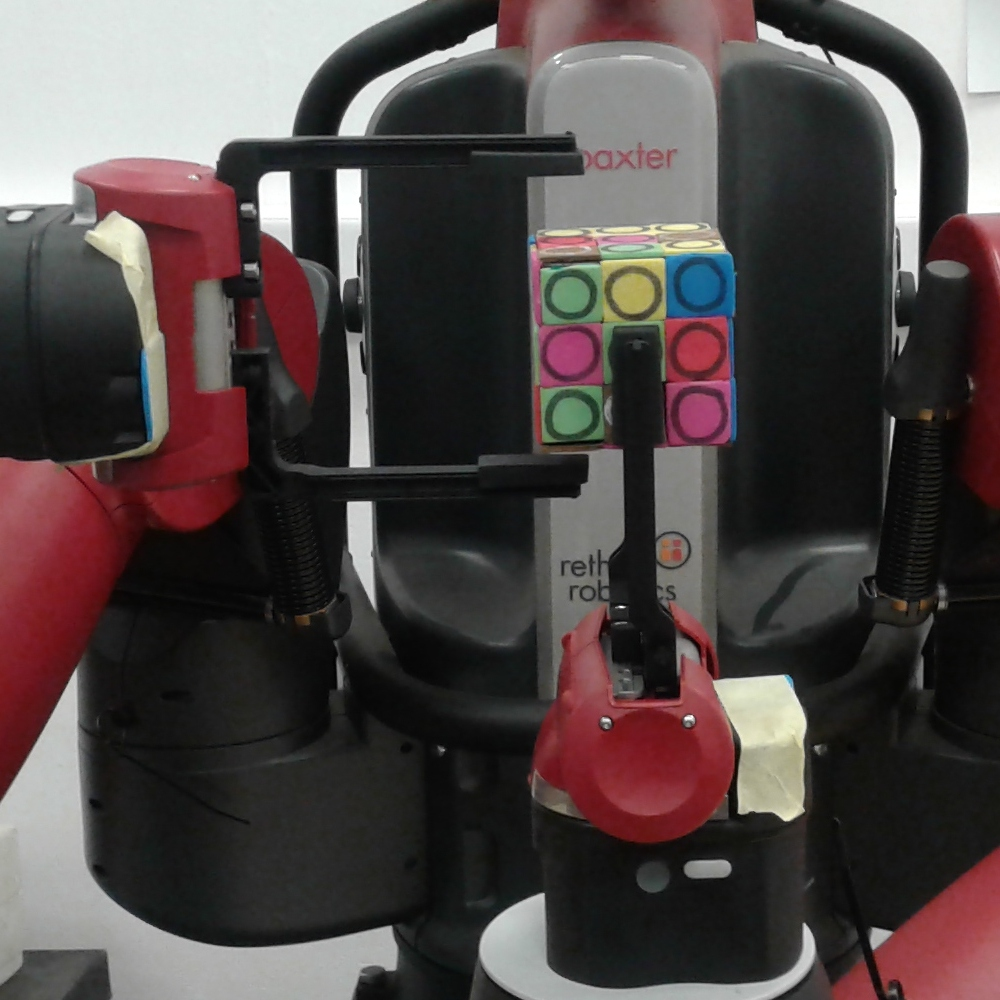
\includegraphics[width=0.30\textwidth]{figures/small_move_F}
	}%
	\hfill
	\subcaptionbox{Rotación cara \textit{D}}{%
		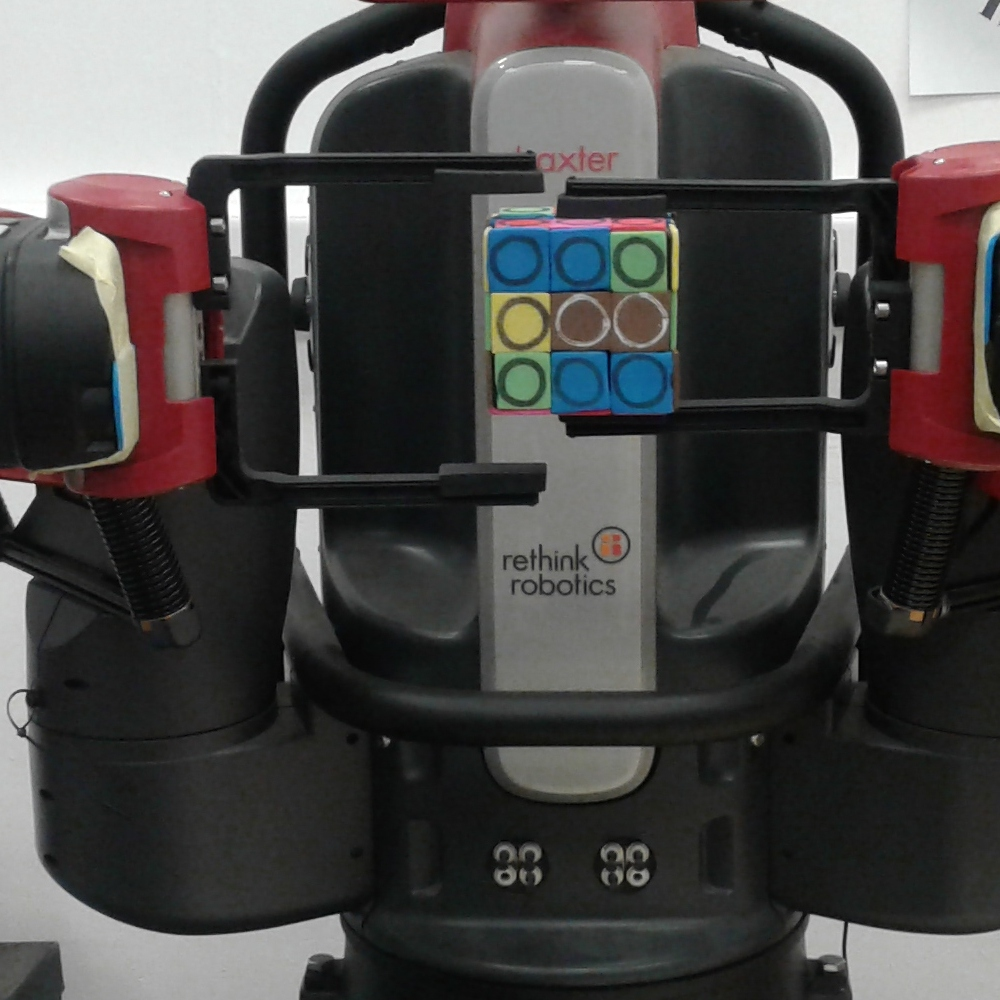
\includegraphics[width=0.30\textwidth]{figures/small_move_D}
	}%
	\hfill
	\subcaptionbox{Rotación cara \textit{B}}{%
		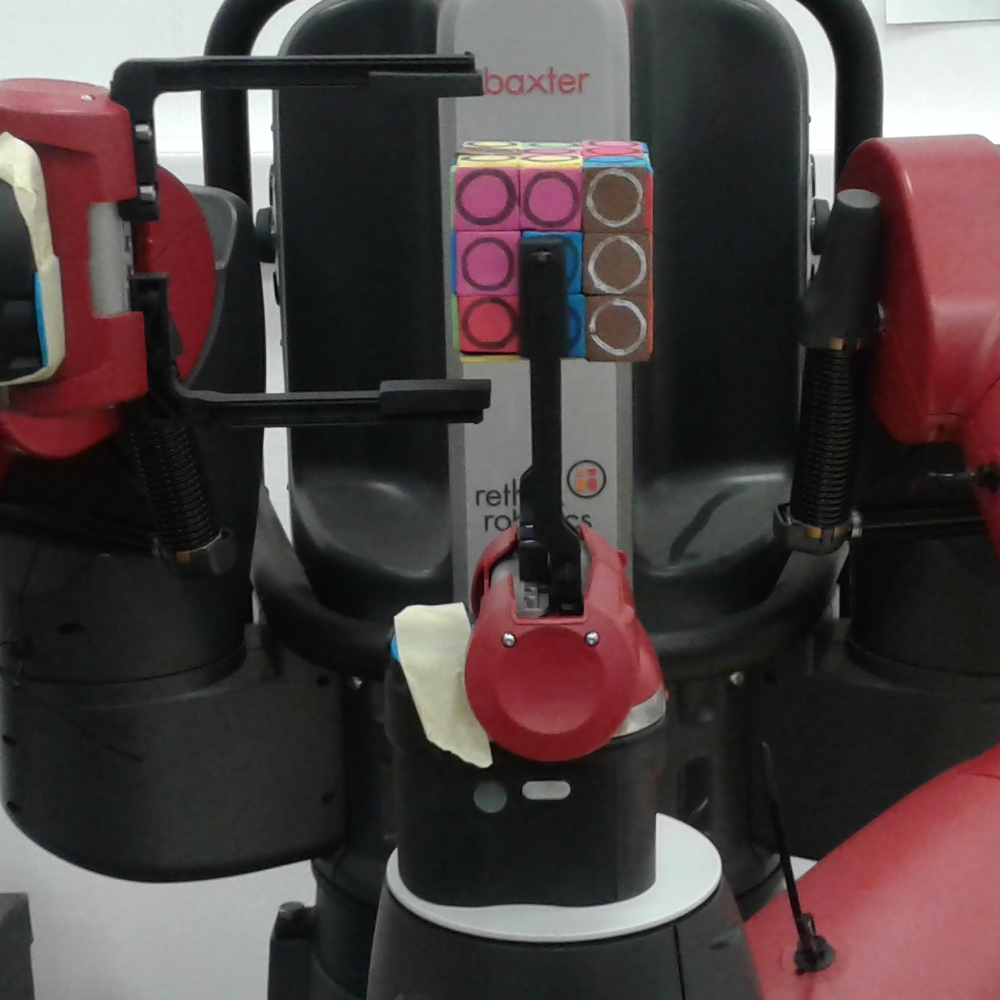
\includegraphics[width=0.30\textwidth]{figures/small_move_B}
	}%
	\caption{Configuraciones del brazo izquierdo para rotaciones.}
	\label{movel}
\end{figure}
\begin{figure}[h!]
	\centering
	\subcaptionbox{Rotación cara \textit{L}}{%
		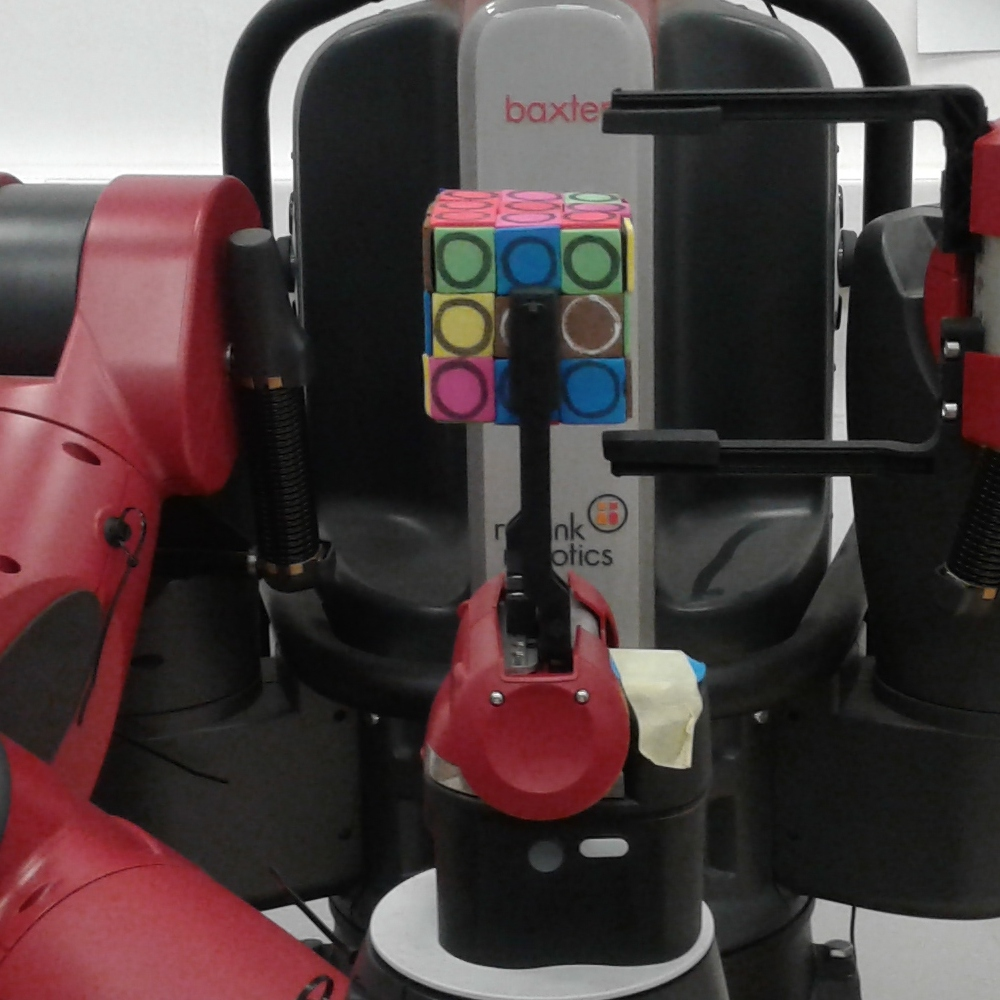
\includegraphics[width=0.30\textwidth]{figures/small_move_L}
	}%
	\hfill
	\subcaptionbox{Rotación cara \textit{U}}{%
		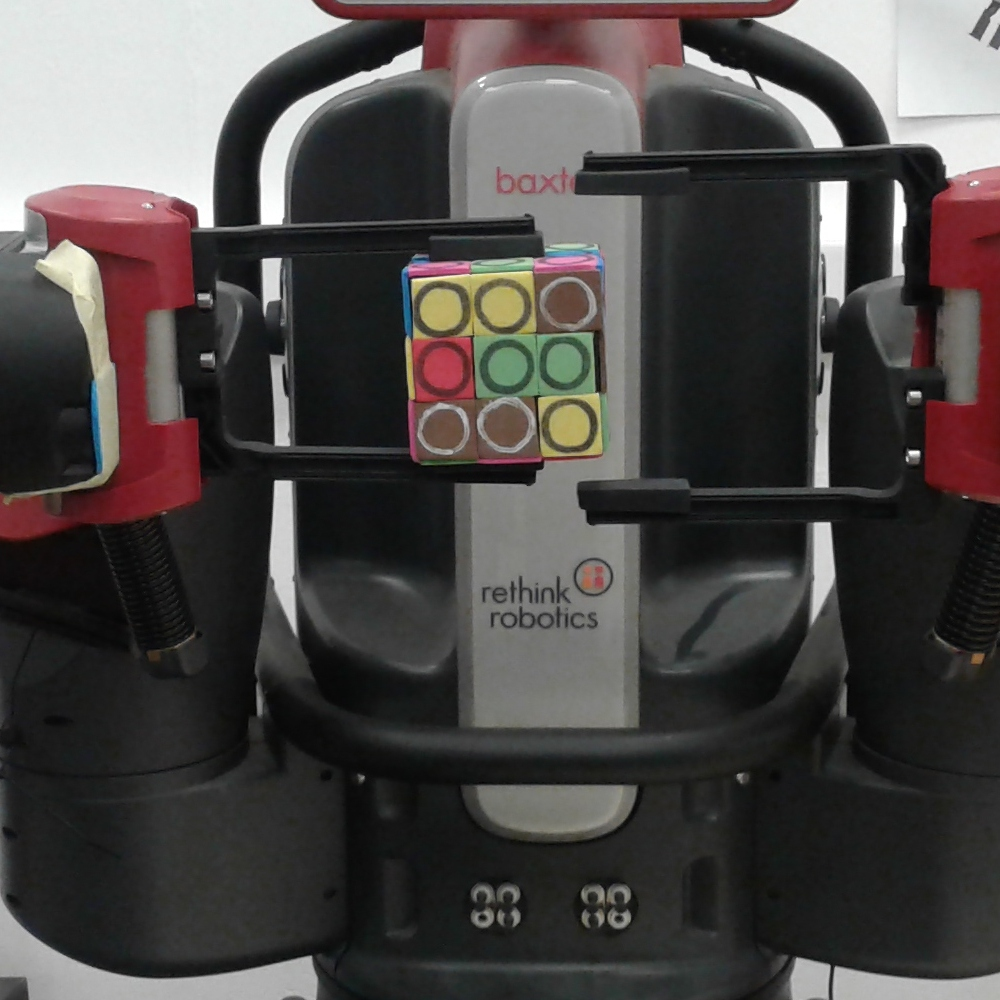
\includegraphics[width=0.30\textwidth]{figures/small_move_U}
	}%
	\hfill
	\subcaptionbox{Rotación cara \textit{R}}{%
		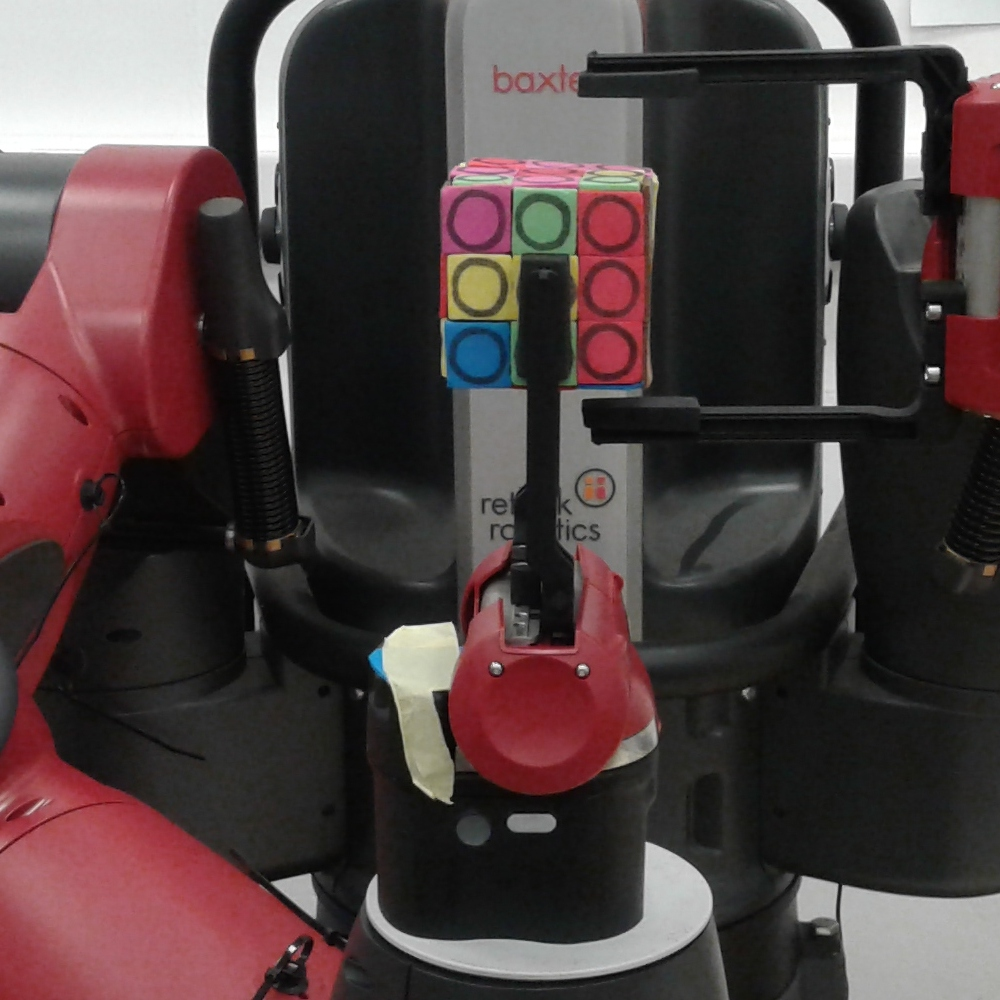
\includegraphics[width=0.30\textwidth]{figures/small_move_R}
	}%
	\caption{Configuraciones del brazo derecho para rotaciones.}
	\label{mover}
\end{figure}
Otra diferencia es que en este paso se agregan posiciones intermedias al acercar el brazo libre a la posición del cubo, para que el servicio de cinemáticas inversas prefiera movimientos paralelos y no cause colisiones no deseadas.

Para efectuar una rotación de alguna cara, la secuencia de pasos es:
\begin{enumerate}
	\item Brazo que sostiene el cubo se mueve a una posición definida en función de la cara que será rotada (especificada mediante ángulos de articulaciones directamente).
	\item Brazo libre se mueve a una posición cercana a la cara a rotar del cubo, pero no lo suficiente para agarralo (especificada mediante IK).
	\item Brazo libre se mueve a una posición aún mas cercana a la cara a rotar del cubo, lo suficiente para agarralo (IK, movimiento paralelo).
	\item Gripper de brazo libre se cierra.
	\item Brazo libre rota articulación de su muñeca en el ángulo deseado (ángulos directos).
	\item Gripper de brazo libre se abre.
	\item Brazo libre se aleja del brazo que sostiene el cubo para permitir libertad en los movimientos siguientes (IK, seguido de ángulos directos).
\end{enumerate}

\subsubsection{Cambio de mano}
Este paso utiliza ángulos directos y cinemáticas inversas. Las posiciones para realizar este paso son las mismas de los brazos ocupados para los movimientos \textit{U} y \textit{R} respectivamente (ambos brazos horizontales, apuntandose a si mismos), con la diferencia de que el brazo izquierdo tiene un desplazamiento de $90$ grados. Así, cuando se cambia el brazo de la mano izquierda a la derecha, se liberan las caras \textit{L}, \textit{R} y \textit{U}, pero se bloquean las caras \textit{F}, \textit{B} y \textit{L}, y viceversa.

\begin{figure}[h!]
	\centering
	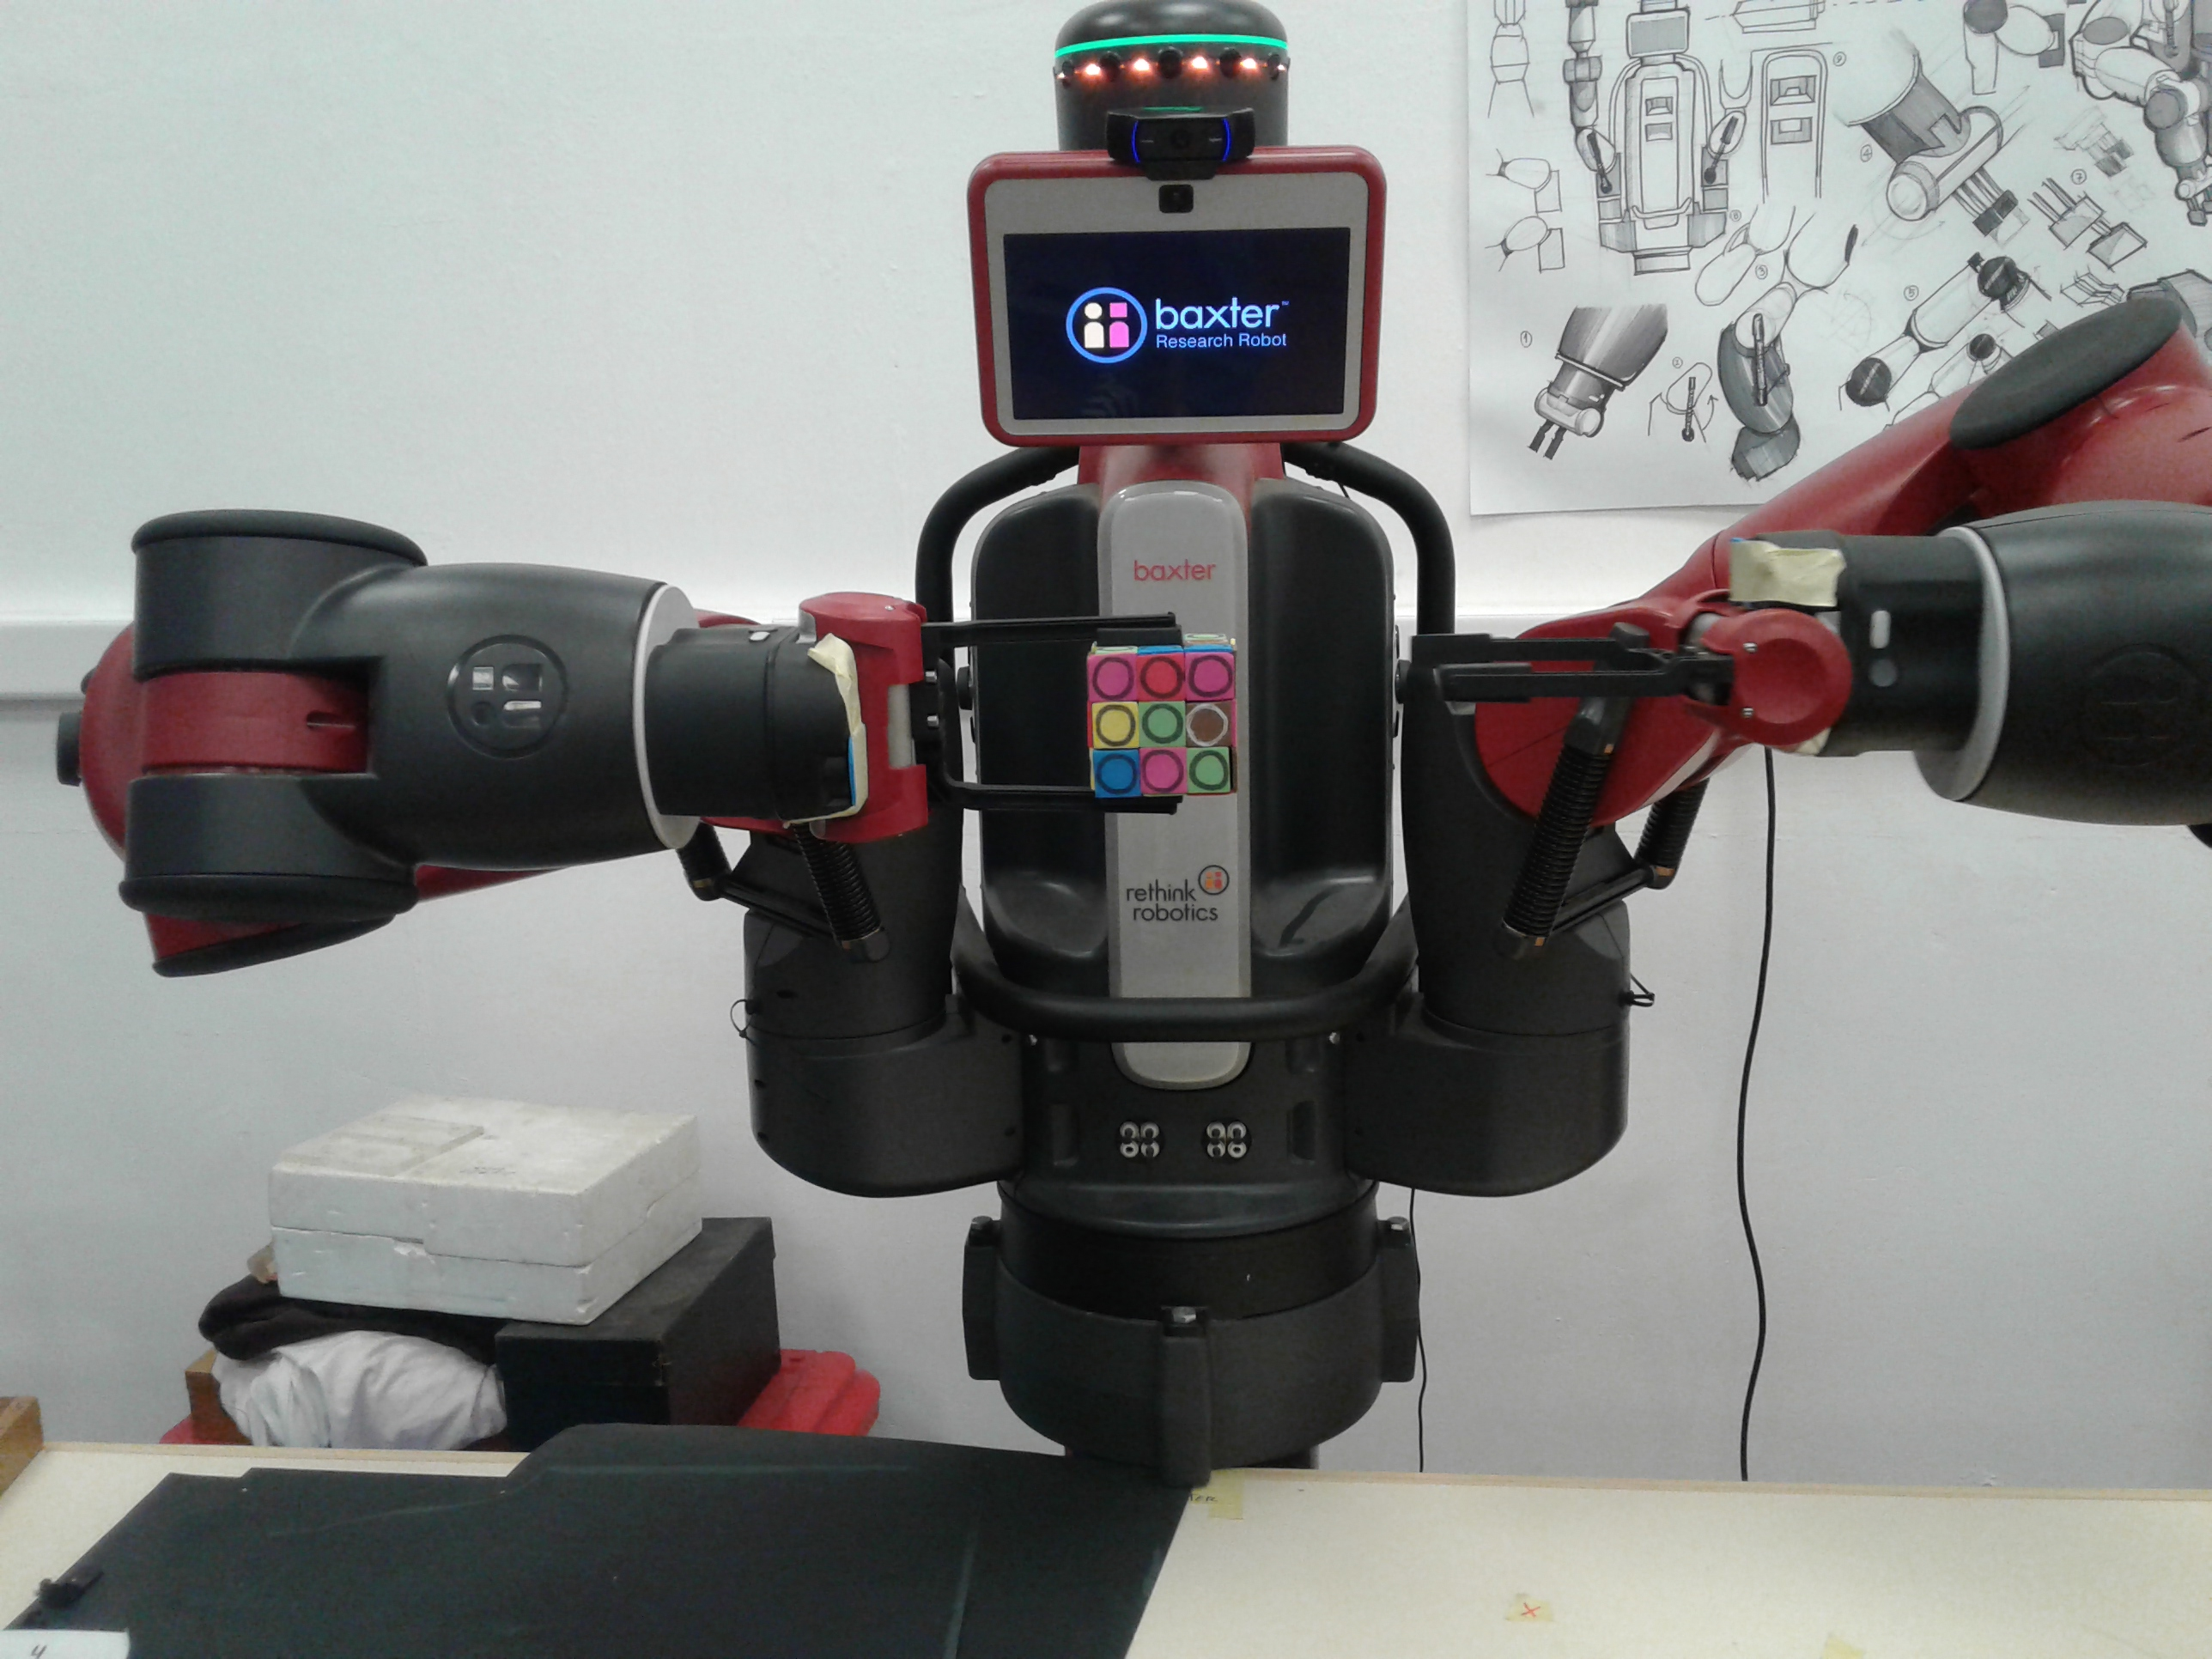
\includegraphics[scale=0.1]{figures/switch}
	\caption{Cambio de mano.}
	\label{switch}
\end{figure}

Al tener 3 caras libres por brazo, no suele ser necesario realizar muchos cambios de mano para llevar a cabo una secuencia de giros. Sin embargo, en el peor caso siempre se tendrá tantos cambios de mano como rotaciones se vaya a realizar.

\subsection{Visión}
Estos módulos se encargan de obtener el estado del cubo. Es la parte más compleja del sistema, en términos de la cantidad de submódulos involucrados.
\subsubsection{Preparaciones previas en el robot}
Si bien Baxter posee cámaras en sus $2$ manos y en su cabeza, la calidad de la imagen que se obtiene usándolas es insatisfactoria. Se decidió entonces utilizar una cámara externa, en concreto, una Logitech C920\cite{logitech}, la cual se ubicó encima de la cámara de la cabeza del robot. Ésta fue conectada directamente al computador desde donde se ejecuta el programa principal, pues a pesar de que el robot tiene interfaces USB (que permite el uso de joysticks entre otros dispositivos) no se encontró documentación ni códigos de ejemplo respecto del uso de cámaras externas.
\begin{figure}[h!]
	\centering
	\subcaptionbox{Cámara brazo izquierdo.}{%
		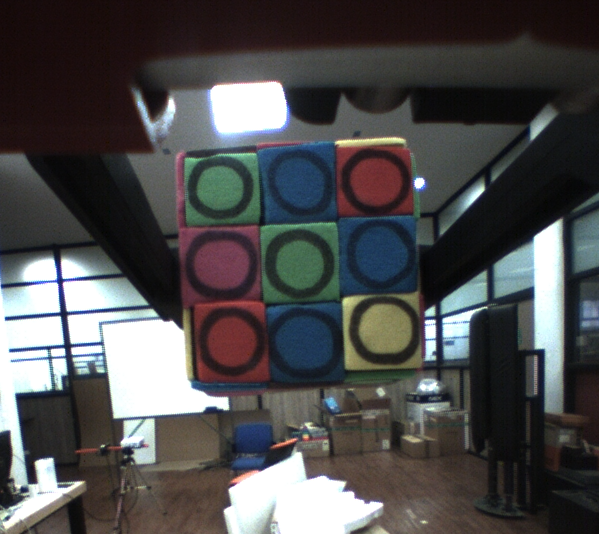
\includegraphics[width=0.24\textwidth]{figures/camara_izq}
	}%
	\hfill
	\subcaptionbox{Cámara brazo derecho.}{%
		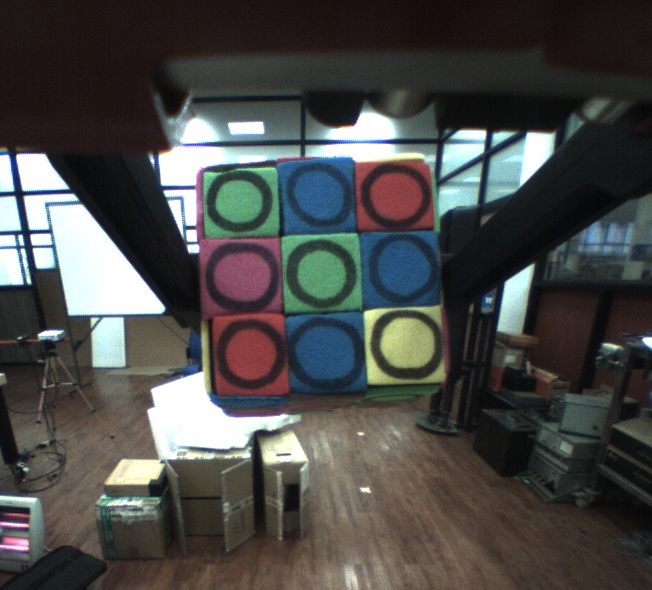
\includegraphics[width=0.24\textwidth]{figures/camara_der}
	}%
	\hfill
	\subcaptionbox{Cámara de la cabeza.}{%
		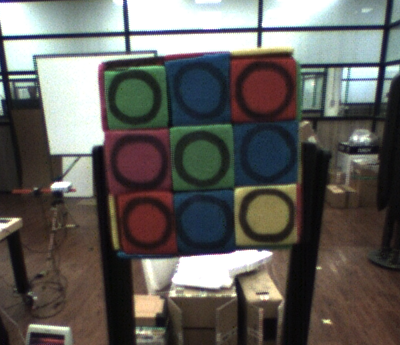
\includegraphics[width=0.24\textwidth]{figures/camara_cabeza}
	}%
	\hfill
	\subcaptionbox{Cámara externa.}{%
	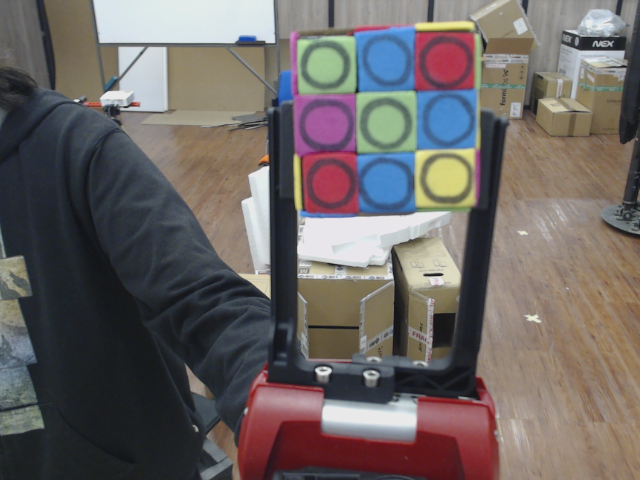
\includegraphics[width=0.24\textwidth]{figures/camara_externa}
	}%
	\caption[Calidad de imagen de las distintas cámaras disponibles.]{Calidad de imagen de las distintas cámaras disponibles. Las imágenes tomadas por las cámaras del robot presentan ruido en forma de un patrón mallado, mientras que la externa no tiene este problema.}
	\label{camaras}
\end{figure}

\subsubsection{Preparaciones previas cubo}
El cubo fue cubierto con etilvinilacetato, mejor conocido como goma EVA. Esto cumple varios objetivos. En primer lugar, es un material que refleja la luz más difusamente que el plástico de los stickers del cubo, por lo que los colores capturados por la cámara tienden a ser más uniformes y se evitan las reflexiones especulares en la imagen. La diferencia es notable y se puede apreciar en la figura~\ref{luz}.

\begin{figure}[h!]
	\centering
	\subcaptionbox{Luz sobre el plástico. Algunos facelets podrian ser erróneamente detectados como blanco.}{%
	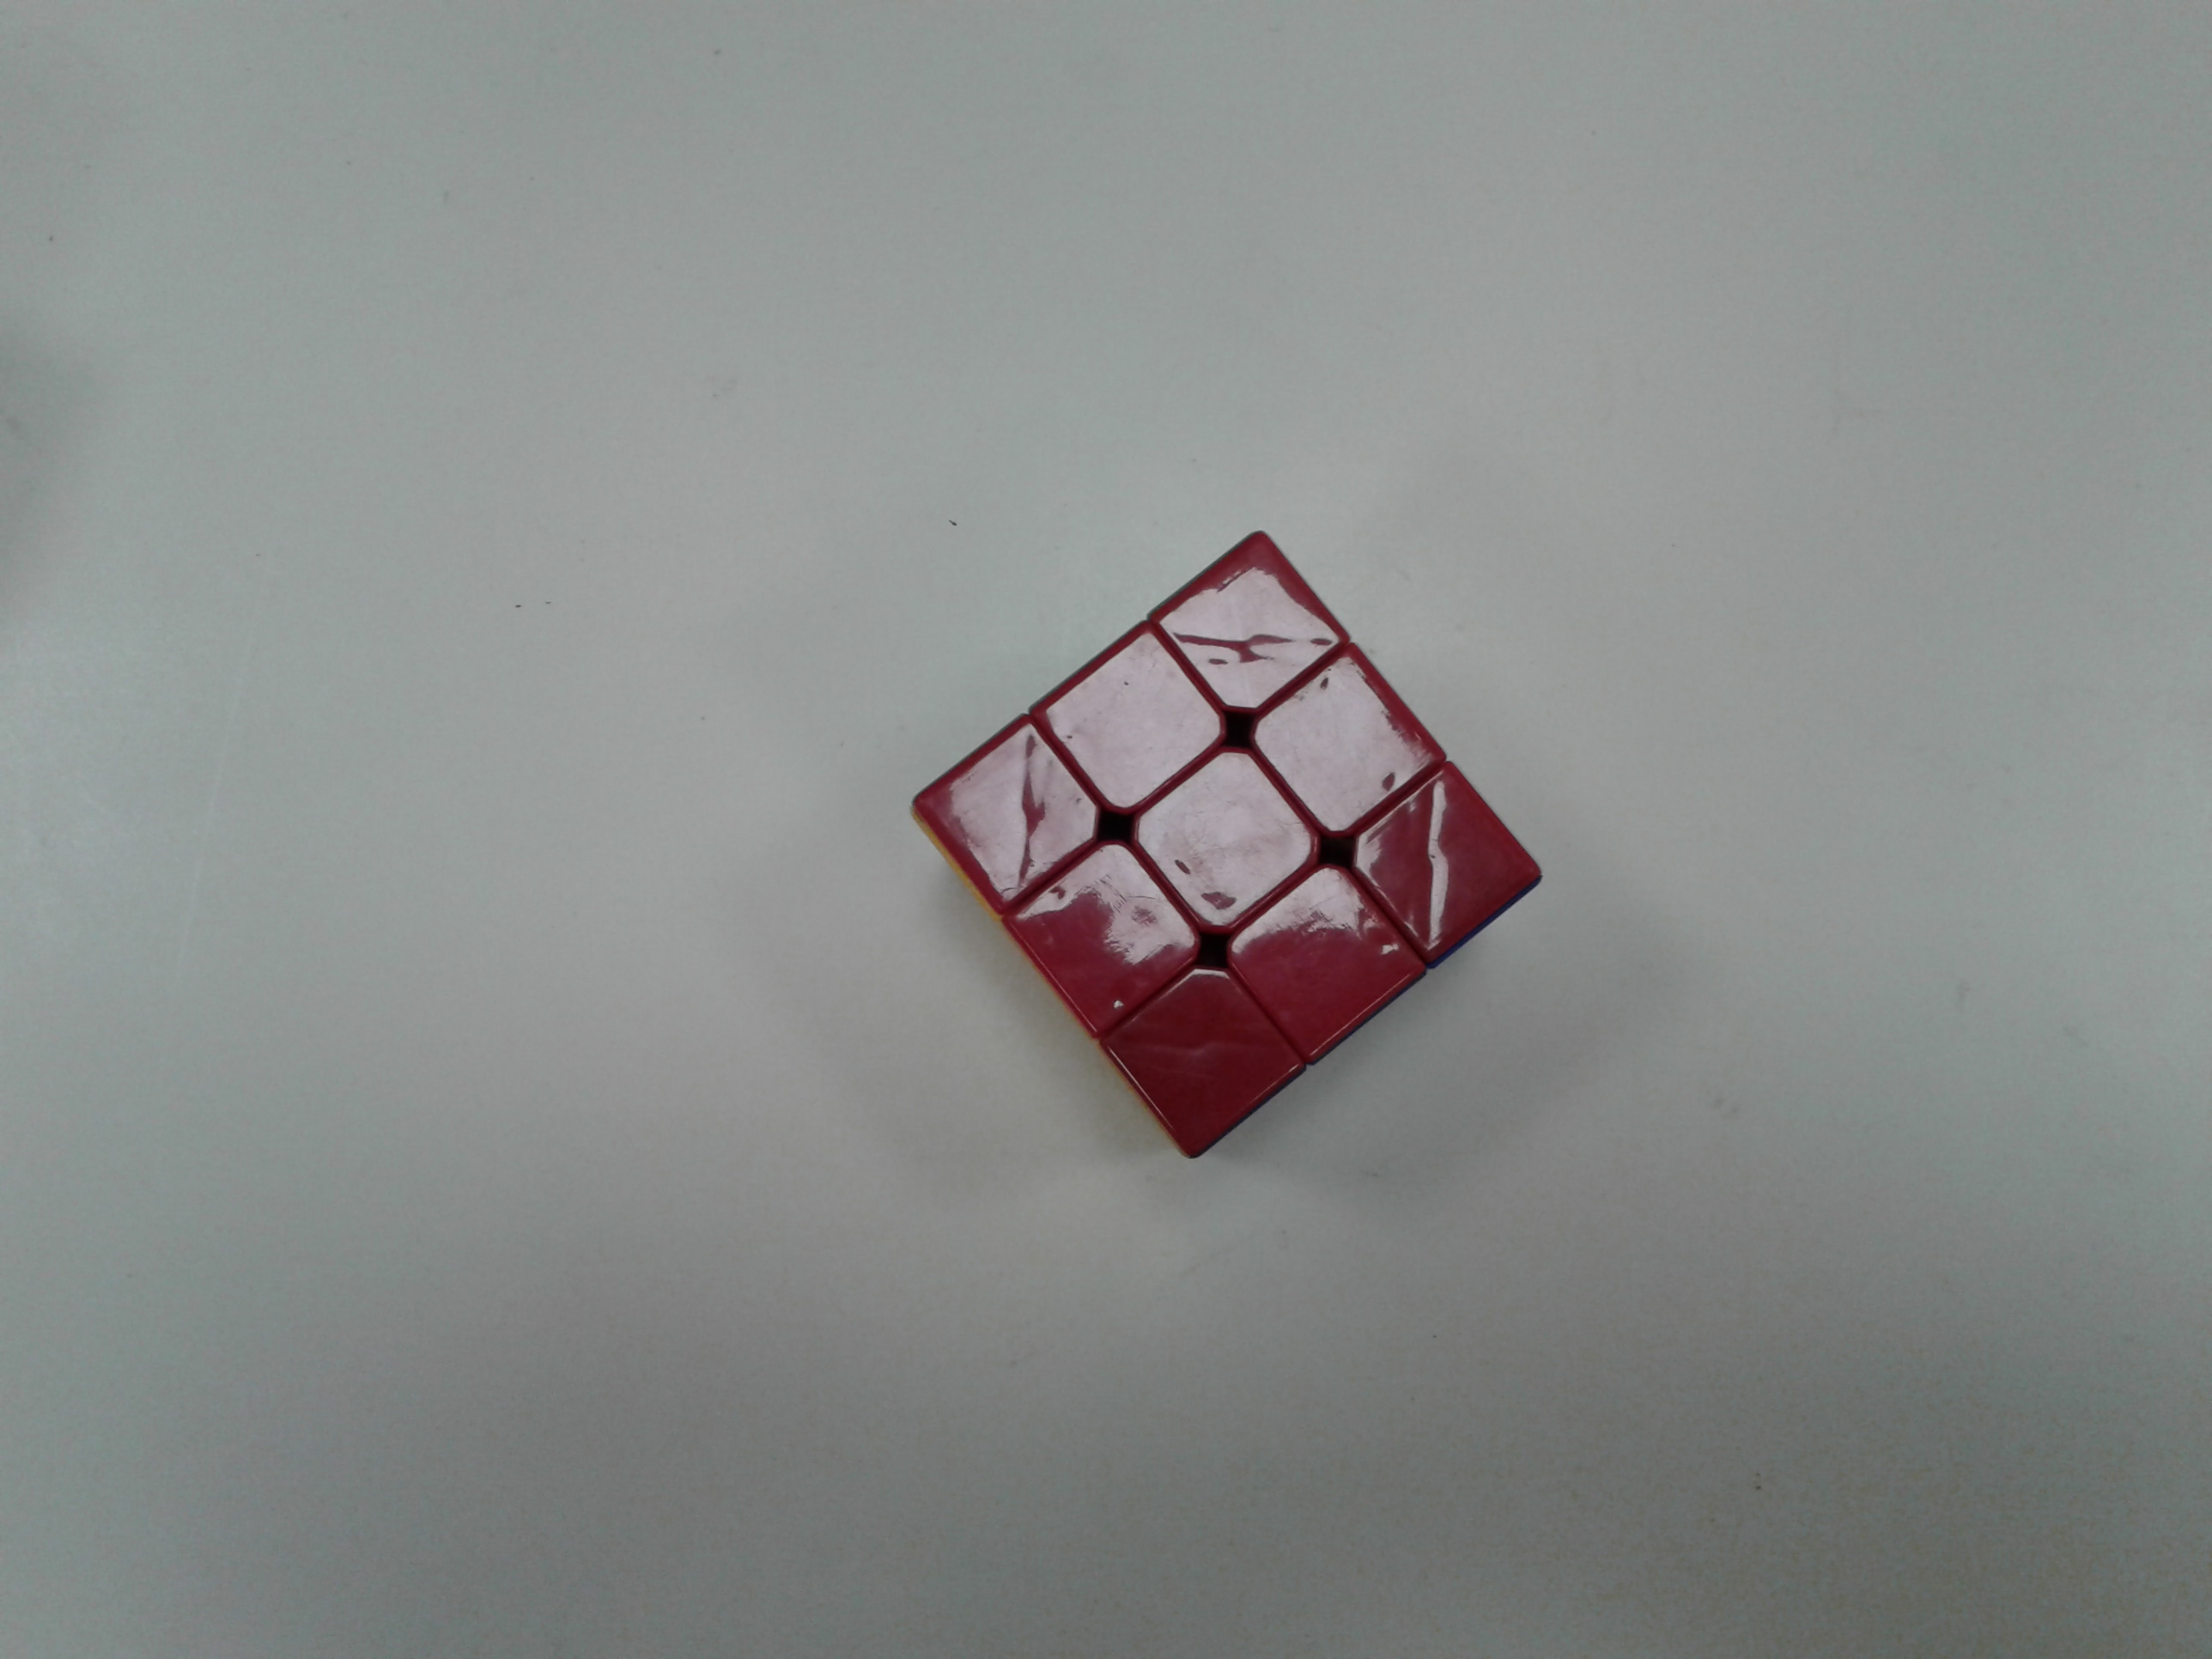
\includegraphics[width=0.48\textwidth]{figures/luz_plastico}
	}%
	\subcaptionbox{Luz sobre la goma EVA. }{%
	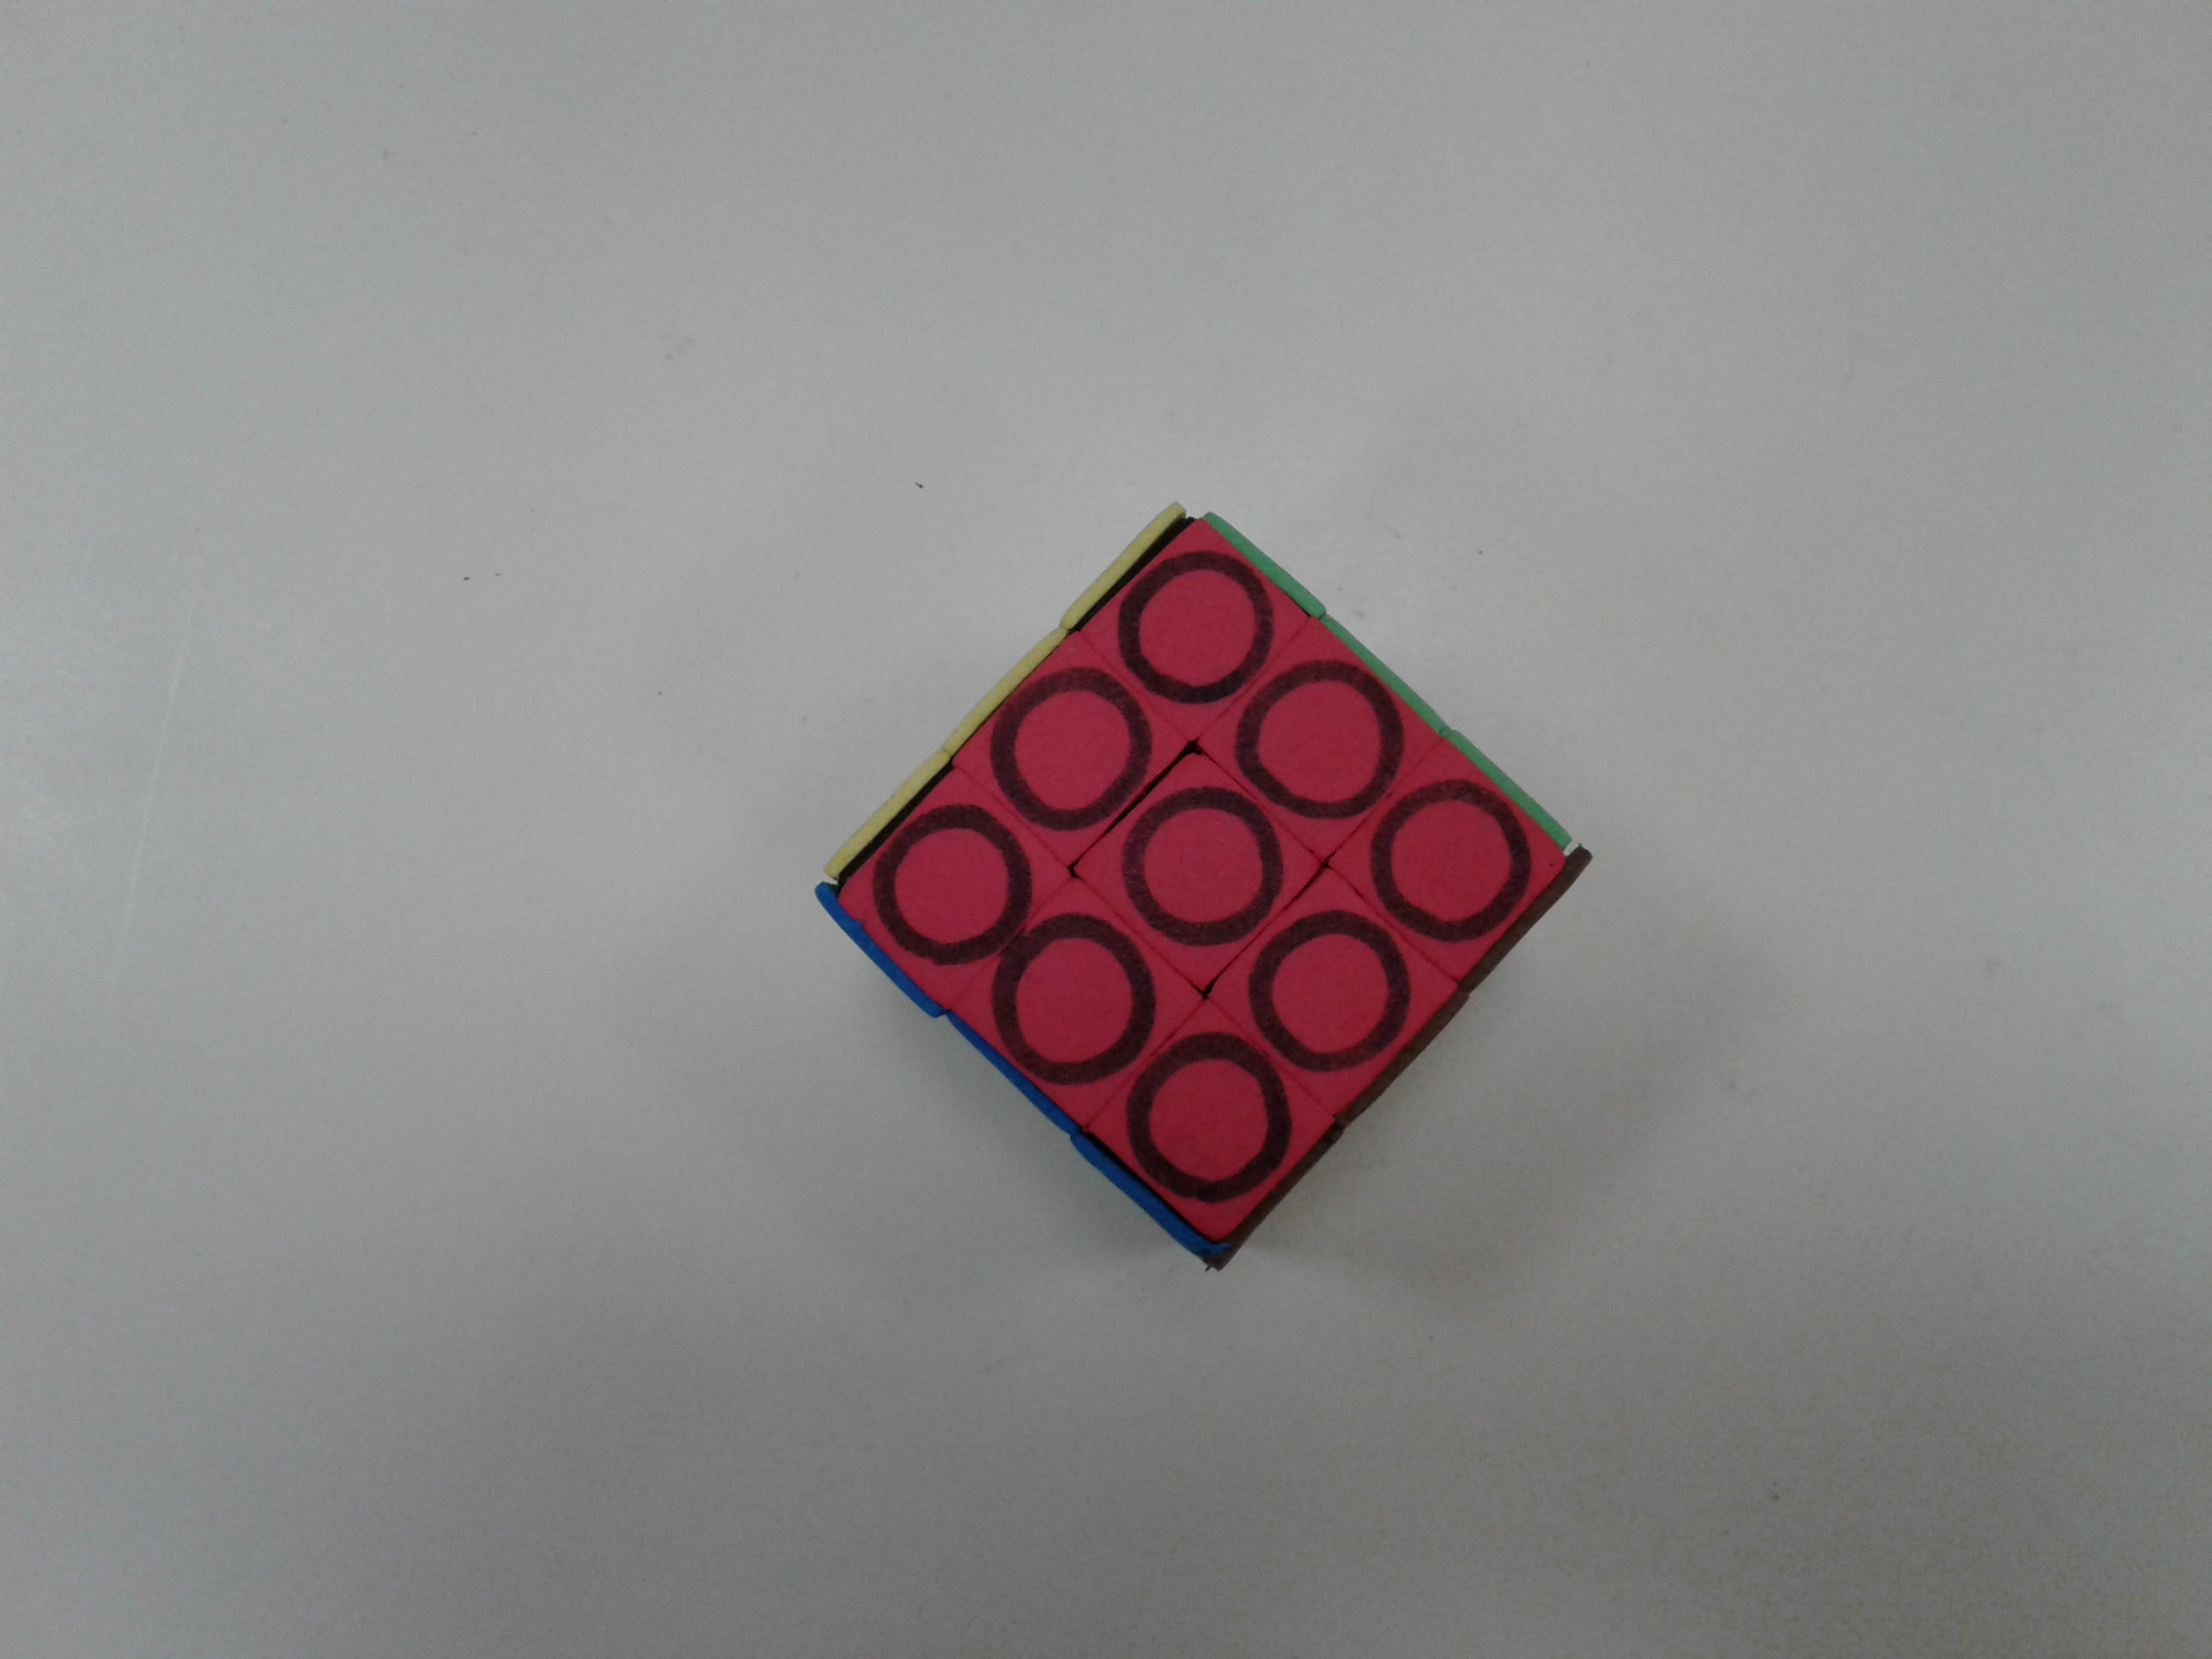
\includegraphics[width=0.48\textwidth]{figures/luz_goma_eva}
	}%
	\caption{Difusión de luz en ambos materiales.}
	\label{luz}
\end{figure}

En segundo lugar, la goma EVA aumenta el roce entre los grippers y el cubo, ya que el plástico original tendía a deslizarse con mayor facilidad. Por último pero no menos importante, provee algo de protección cuando el cubo es maltratado por los movimientos poco delicados del robot.

Los colores de goma EVA utilizados fueron rojo, azul, verde, amarillo, rosado y marrón, correspondientes a los mismo colores originales con excepción de los $2$ últimos (naranja y blanco, originalmente), pues no se disponía de naranja y  el blanco se ensucia bastante luego de muchas manipulaciones.

Sobre cada facelet del cubo se dibujó un círculo con un marcador permanente, negro, para denotar el borde de las regiones de interés (los facelets) con un color que contrastase los colores claros de la goma EVA, con excepción del marrón, cuyos círculos fueron dibujados con color blanco para mayor contraste.

\begin{figure}[h!]
	\centering
	\subcaptionbox{Cubo original, caras \textit{U} \textit{R} y \textit{F}.}{%
	\includegraphics[width=0.35\textwidth]{figures/plastico_urf}
	}%
	\hfill
	\subcaptionbox{Cubo original, caras \textit{D} \textit{L} y \textit{B}.}{%
	\includegraphics[width=0.35\textwidth]{figures/plastico_dlb}
	}%
	\hfill
	\subcaptionbox{Cubo cubierto, caras \textit{U} \textit{R} y \textit{F}.}{%
	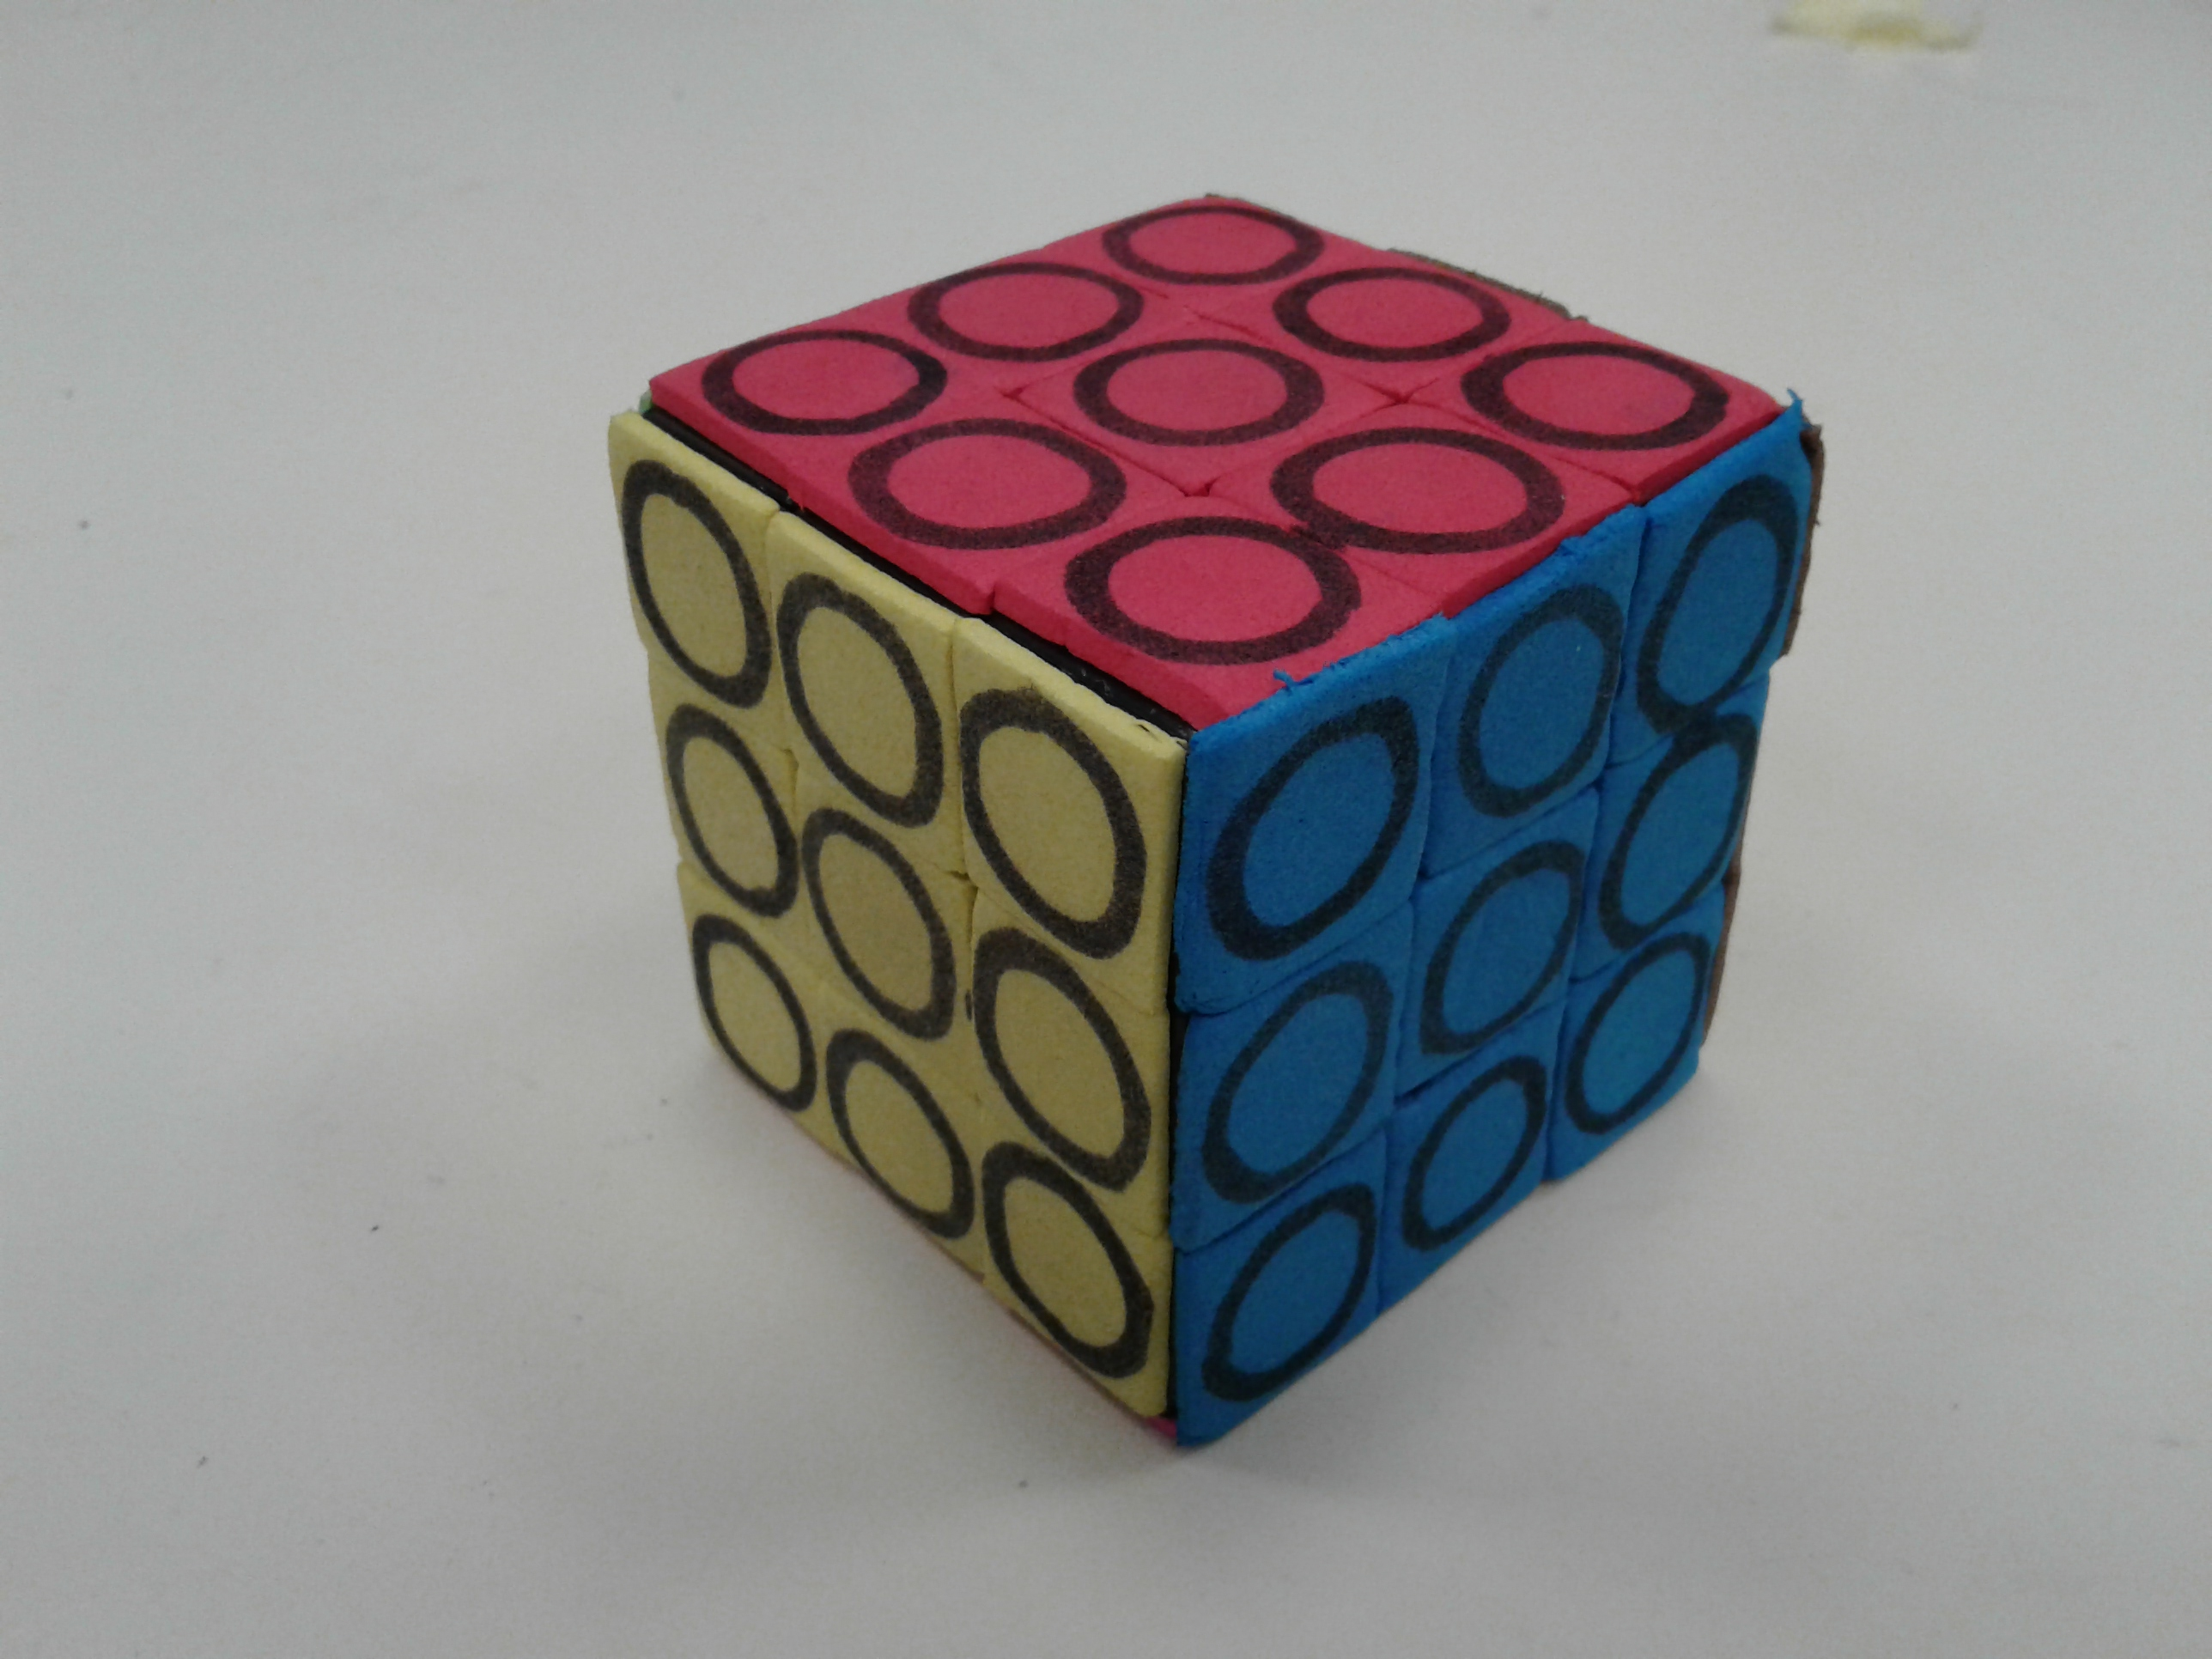
\includegraphics[width=0.35\textwidth]{figures/goma_eva_urf}
	}%
	\hfill
	\subcaptionbox{Cubo cubierto, caras \textit{D} \textit{L} y \textit{B}.}{%
	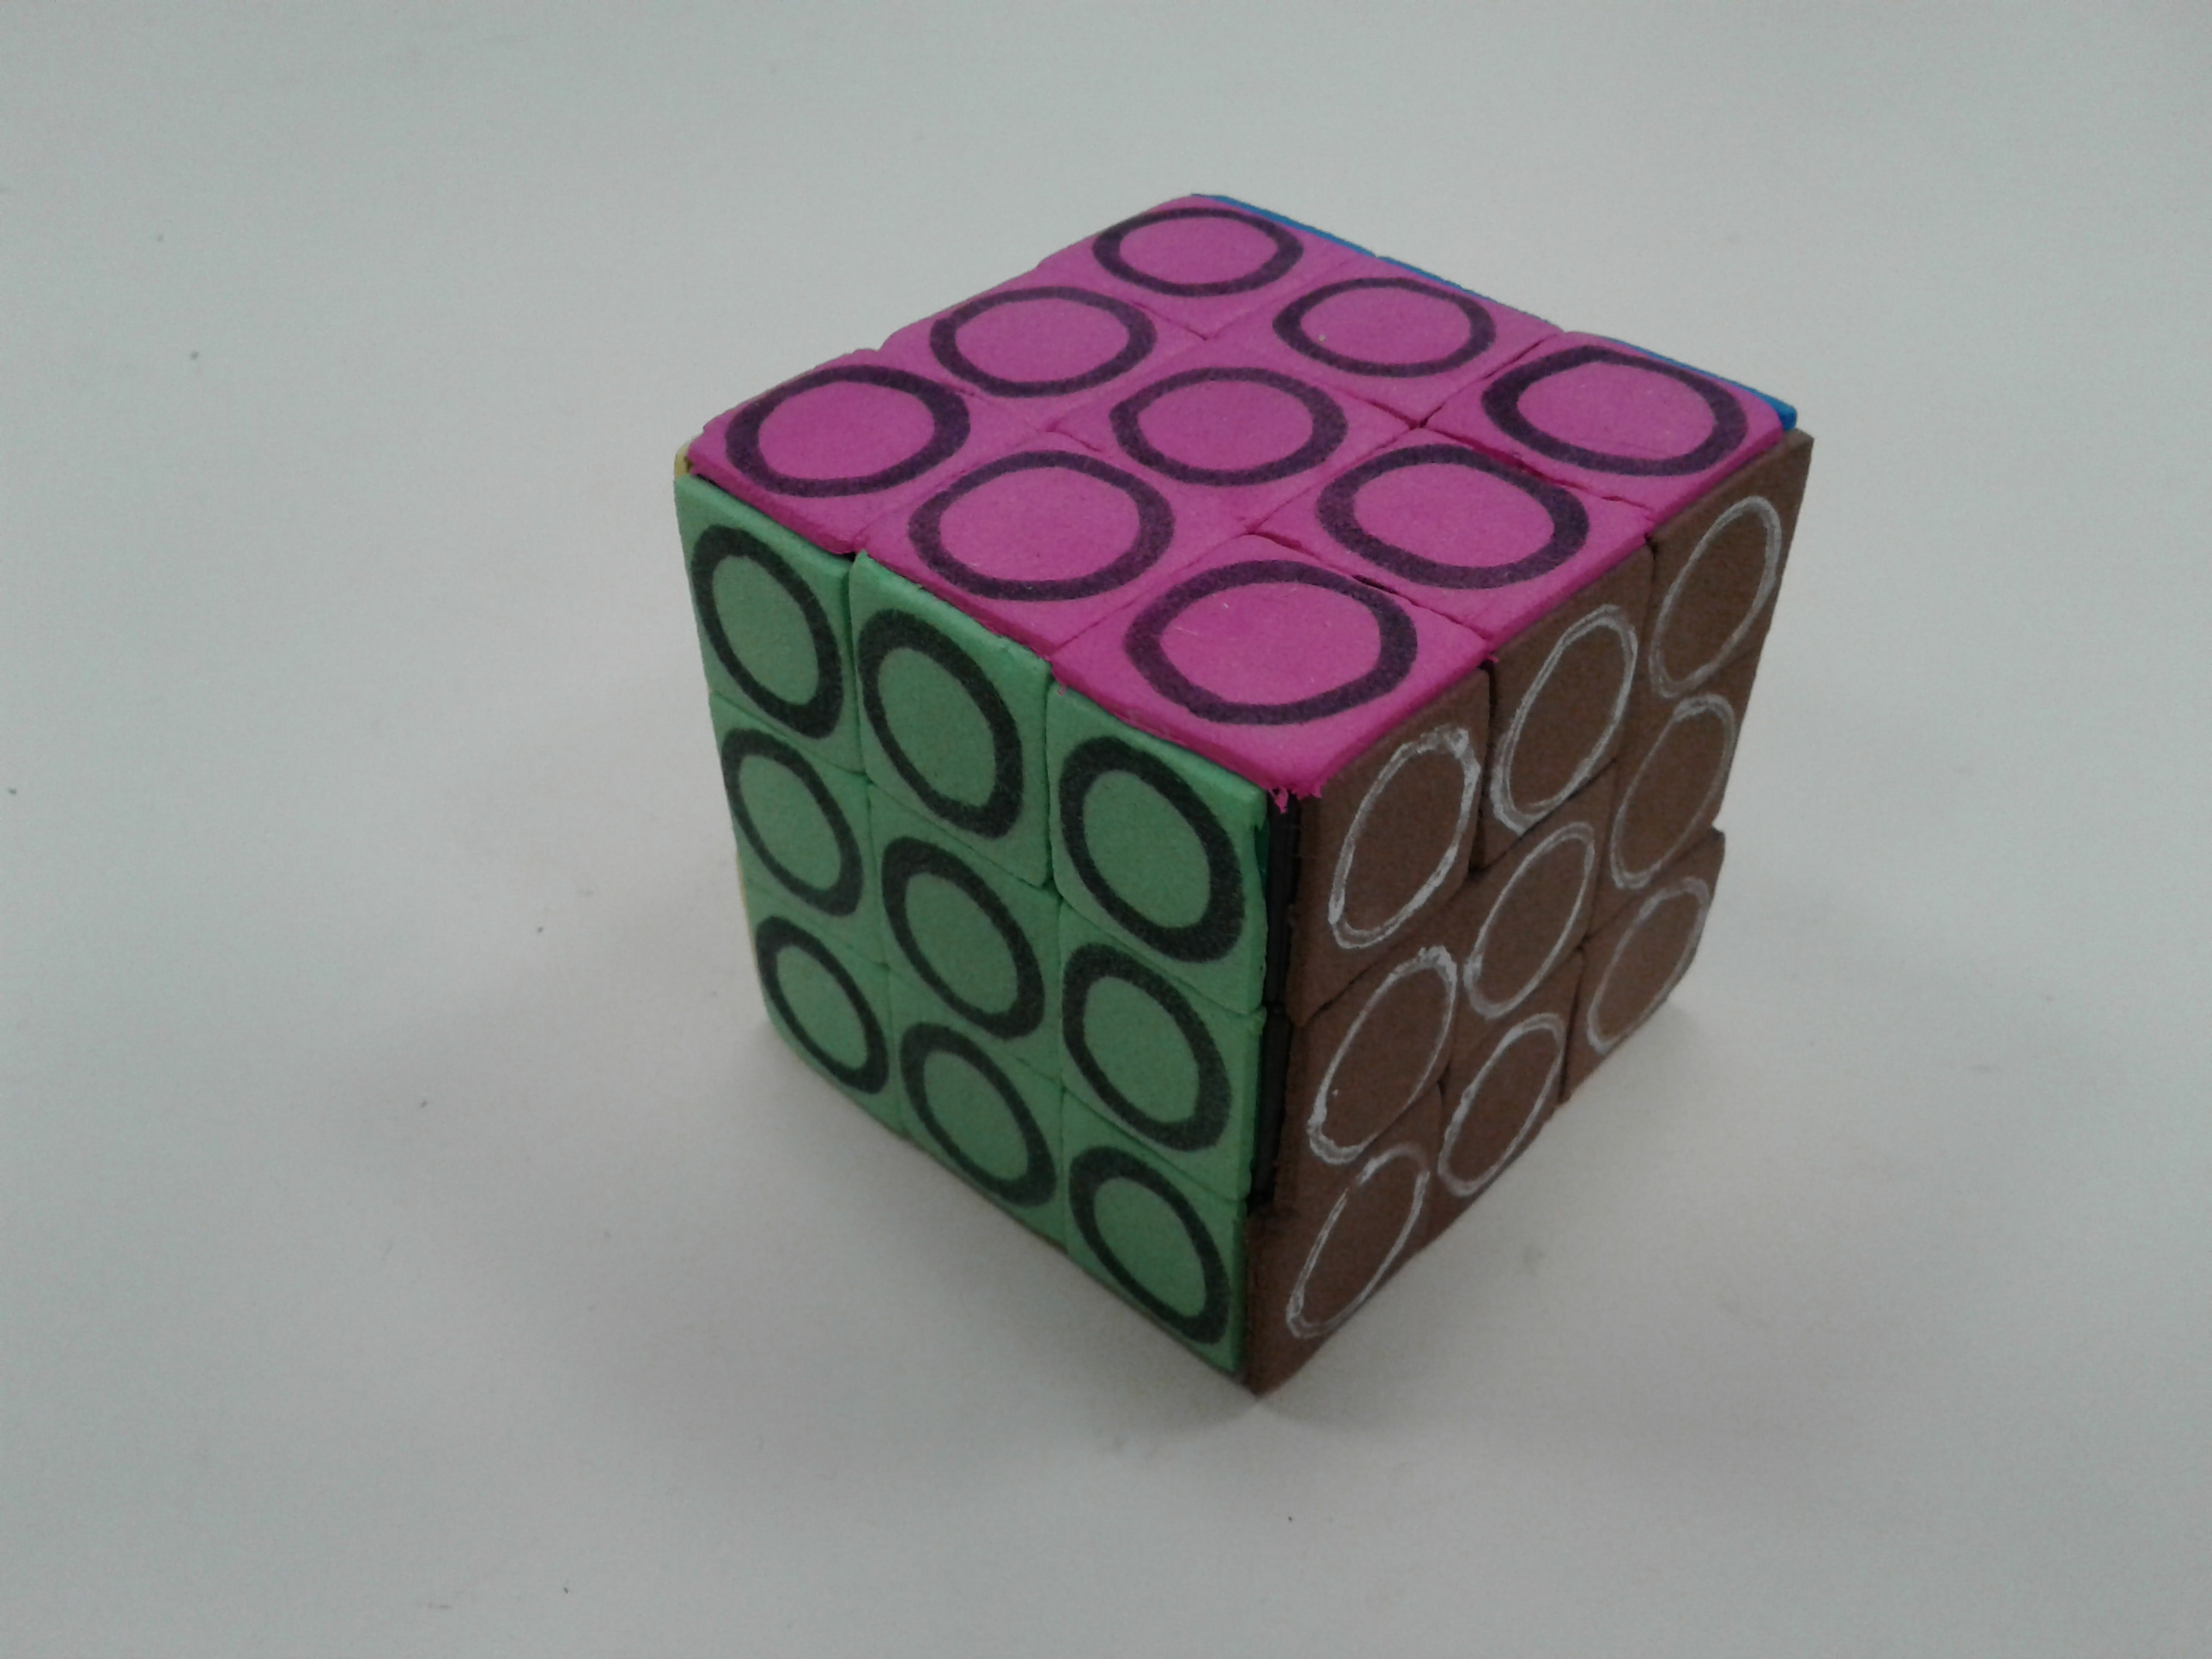
\includegraphics[width=0.35\textwidth]{figures/goma_eva_dlb}
	}%
	\caption{Colores del cubo de Rubik usado.}
	\label{colorescubo}
\end{figure}

\subsubsection{Círculos de Hough}
Una vez que el manipulador acerca el cubo a la cámara, se capturan fotos de cada cara. Sobre cada una de estas $6$ imágenes, se aplica el algoritmo de Hough para detección de círculos, provisto por la biblioteca de OpenCV \textit{HoughCircles} que implementa dicho algoritmo. El método itera hasta que encuentra exactamente $9$ círculos en cada imagen, entregando sus centros y radios respectivos.

\begin{figure}[h!]
	\centering
	\subcaptionbox{Detección incorrecta, faltan círculos.}{%
		\includegraphics[width=0.35\textwidth]{figures/small_circulos_pocos}
	}%
	\hfill
	\subcaptionbox{Detección incorrecta, sobran círculos.}{%
		\includegraphics[width=0.35\textwidth]{figures/small_circulos_muchos}
	}%
	\hfill
	\subcaptionbox{Detección correcta.\label{deteccioncorrecta}}{%
	\includegraphics[width=0.35\textwidth]{figures/small_circulos}
	}%
	\caption{Identificación de círculos.}
	\label{circulos}
\end{figure}

La transformada de Hough\cite{hough} es una técnica para extracción de características en imágenes, inicialmente concebida para detectar líneas, pero posteriormente se generalizó para detectar círculos o elipses. Una ventaja de utilizar esta transformación es que es muy robusta, pudiendo detectar círculos imperfectos, incluso cuando están parcialmente ocultos por un objeto entre la cámara y el círculo. Su cómputo y en particular su implementación en OpenCV es bastante rápida, sin embargo no es perfecta. Dependiendo del ambiente de la imagen y los parámetros utilizados se pueden obtener falsos positivos, o falsos negativos, como se ve en la figura \ref{circulos}.

Mediante ensayo y error se obtubieron parámetros lo suficientemente buenos para la transformada de Hough. Estos fueron radio mínimo y máximo de $10$ y $35$ píxeles para los círculos, con una distancia mínima entre ellos de $30$ píxeles. Otros dos parámetros correspondientes a umbrales que controlan la cantidad potencial de círculos (\texttt{param1} y \texttt{param2}) se dejaron en $80$ y $30$ respectivamente.

\subsubsection{Colores representantes}
Una vez se tienen los $54$ círculos, se procede a extraer un color representativo de la región encerrada por cada uno. Se decidió usar la mediana RGB, pues en el caso de una detección imperfecta de un círculo (como el facelet rosado de la figura \ref{deteccioncorrecta}) no se quiere que el borde del círculo afecte al color representante. Para mayor comodidad en la iteración, se utilizó como región un cuadrado inscrito en un círculo en lugar del círculo completo. Este paso tiene como resultado un vector 54 colores RGB.

\subsubsection{Clasificación}
\begin{figure}[h!]
	\centering
	\subcaptionbox{Espacio de colores RGB.}{%
		\includegraphics[width=0.4\textwidth]{figures/RGB}
	}%
	\hfill
	\subcaptionbox{Espacio de colores HSV.}{%
		\includegraphics[width=0.4\textwidth]{figures/HSV}
	}%
	\caption[Espacios de colores.]{En RGB, los colores rojo, verde y azul corresponden a 3 ejes cartesianos. En HSV, el espacio tiene coordenadas cilíndricas, donde los colores ``rojos'' tienen radios similares entre sí, al igual que los ``verdes'', ``azules'' y demás colores.}
	\label{colorspace}
\end{figure}
Para identificar cuales facelets son del mismo color, independientemente de cual sea éste, se utilizó un modelo no supervisado para clasificarlos. El algoritmo utilizado fue el de mezcla de gaussianas (Gaussian Mixture Model, o \textit{GMM})\cite{gmm}, con 6 componentes. Las características usadas fueron las componentes matiz y saturación de la conversión de espacio RGB (Red, Green, Blue)\cite{rgb} al espacio HSV (Hue, Saturation, Value)\cite{hsv} de cada uno de los colores representantes de cada facelet.

\begin{figure}[h!]
	\centering
	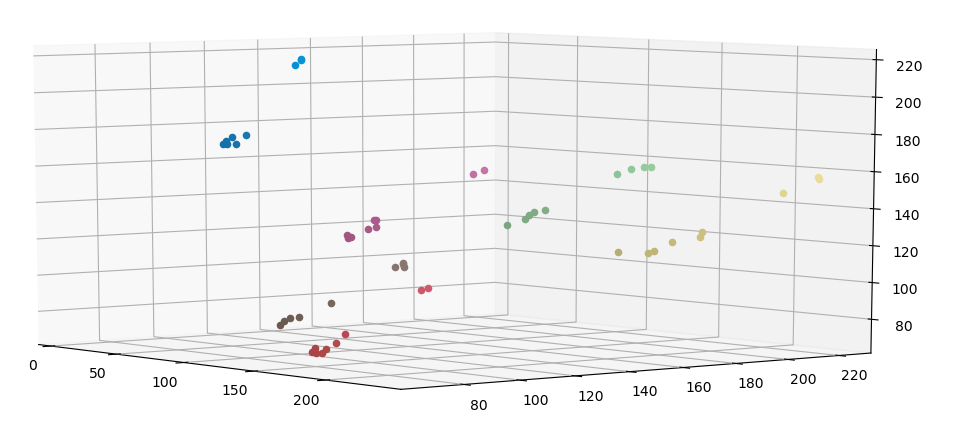
\includegraphics[width=0.8\textwidth]{figures/rgb_3d}
	\caption{Colores representantes en espacio RGB. Los facelets del mismo color se tienden a alinear en rectas que crecen en los 3 ejes.}
	\label{rgb3d}
\end{figure}


Luego de realizar muchos experimentos se observó que la distribución RGB de los colores que vienen de la misma cara se tienden a alinear en rectas (ejemplo de distribución en figura \ref{proyecciones}, en anexo). Después de intentar infructuosamente con varios modelos de agrupamiento (K-Means, KMeans despúes de PCA, KMeans en espacio HSV) se decidió optar por un modelo de mezcla de gaussianas en HSV, pues los colores, con excepción del marrón tienen componentes de matiz muy similares, variando principalmente en su saturación o brillo.

\begin{figure}[h!]
	\centering
	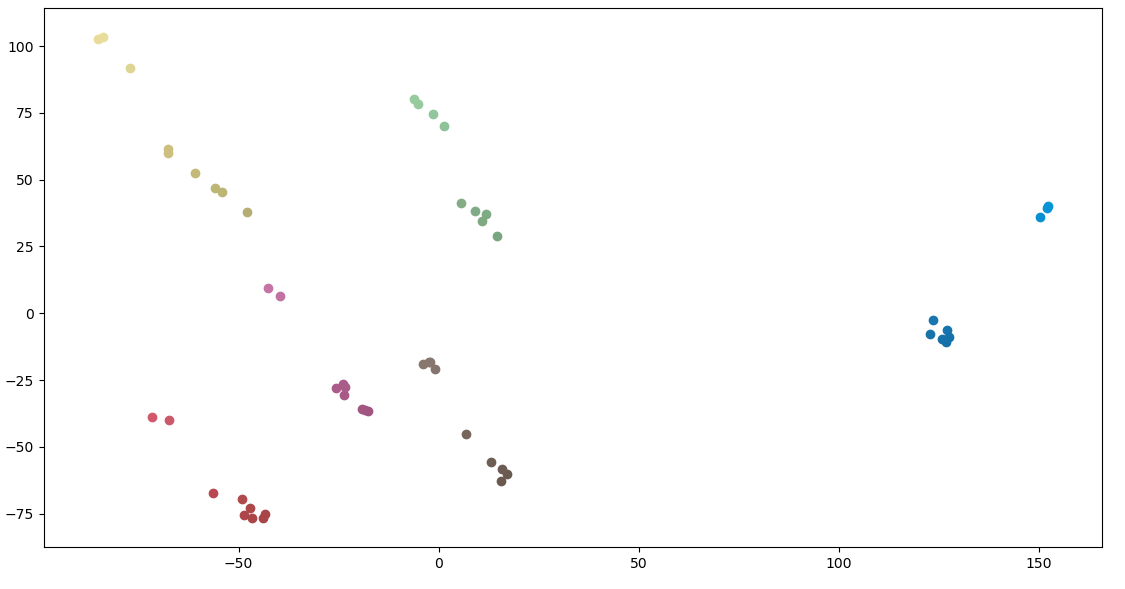
\includegraphics[width=0.8\textwidth]{figures/rgb_pca}
	\caption[Colores representantes, luego de aplicar PCA con 2 componentes]{Colores representantes, luego de aplicar PCA con 2 componentes. Clases no trivialmente separables.}
	\label{rgb3d}
\end{figure}

Aprovechando el hecho de que las piezas centro del cubo no se mueven, se puede saber con certeza de que sus facelets son todos de colores distintos, no así las aristas y esquinas del cubo que pueden moverse libremente a cualquier otra ubicación. Los colores de los centros se utilizaron entonces como las medias iniciales de las gaussianas. Además, se asignaron las probabilidades a priori en 1/6 a cada gaussiana, pues todas las caras tienen la misma cantidad de facelets. Las covarianzas iniciales de cada gaussiana se tomaron con mayor varianza en el eje de saturación que en el de matiz. Esto es simplemente conocimiento previo de la distribución de los datos luego de muchos experimentos. El efecto de elegir las covarianzas de esta forma se muestra en las figuras \ref{gmmgood} y \ref{gmmbad}.

\begin{figure}[h!]
	\centering
	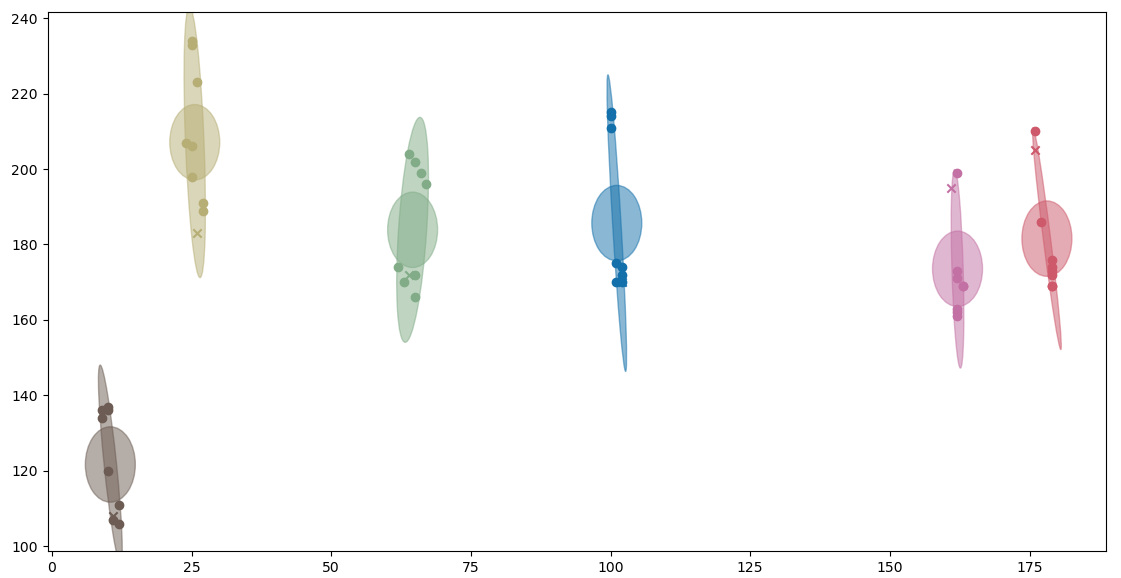
\includegraphics[width=\textwidth]{figures/gmm}
	\caption[Colores representantes en espacio HSV.]{Colores representantes en espacio HSV. Eje horizontal es matiz, eje vertical es saturación. Los puntos marcados con cruces indican los representantes de los centros, y por ende las medias iniciales de las gaussianas. Las elipses grandes son las covarianzas finales, a 2 desviaciones estándar las elipses pequeñnas son las covarianzas iniciales. Esta clasificación es correcta.}
	\label{gmmgood}
\end{figure}

\begin{figure}[h!]
	\centering
	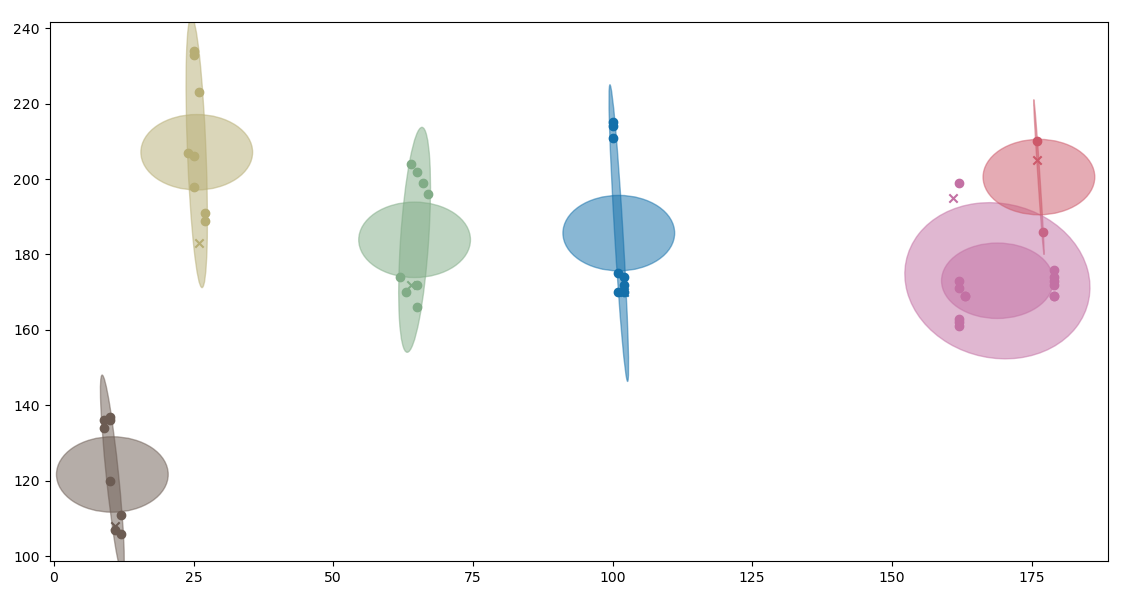
\includegraphics[width=\textwidth]{figures/gmm_bad}
	\caption[Gaussian Mixture Model con covarianzas circulares.]{El mismo caso de la figura~\ref{gmmgood}. Cuando las covarianzas crecen por igual en ambos ejes, ocurren más errores de clasificación, al igual que con KMeans. En particular, puntos rojos fueron incorrectamente clasificados como puntos rosados.}
	\label{gmmbad}
\end{figure}

El algoritmo de agrupamiento de un modelo de mezcla de gaussianas suele calcularse de manera iterativa a partir de una solución inicial, siguiendo el proceso de Expectation-Maximization. Cuando el algoritmo GMM era incializado con el resultado de procesar los puntos con K-Means (como lo hace, por ejemplo el modelo GMM de la biblioteca de Python scikit-learn), se tiende a confundir los colores rojo y rosado, ya que sus matices suelen están más cerca que la distancia en saturación más grande entre 2 rojos o 2 rosados.

Al finalizar este paso, si es que no hubo algún error de clasificación, se tiene un vector de 54 caracteres en el orden dado por la figura \ref{faceletorder}. Así, el caracter \textit{X} en la posición $i$ indica que el facelet $i$ es del mismo color que el centro de la cara \textit{X}. Por ejemplo, para los representantes de las figuras \ref{gmmgood}, el estado resultante es el string \textit{LLLFUBRUBRRFRRUDBBFFUDFUDRRLFFBDDBRRBLUDLFDLFUUUBBLDDL}.


\subsection{Resolución}
Para la fase de resolución se utilizó el algoritmo de $2$ fases de Kociemba.
Este algoritmo encuentra soluciones a cualquier configuración del cubo mediante una búsqueda exhaustiva, realizada en dos pasos.

En la primera fase, se lleva la permutación actual a algún estado en la que todas las piezas arista y esquina tengan orientación igual a cero (ver figura \ref{orientation}). La segunda fase lleva dicha configuración -sin orientaciones- al estado resuelto.

\begin{figure}[h!]
	\centering
	\includegraphics[width=0.5\textwidth]{figures/orientacion}
	\caption[Definición de orientación.]{La orientación de una pieza del cubo se define con respecto a un sistema de referencia dado por los facelets marcados en blanco. Si el facelet marcado de una pieza coincide con la referencia, entonces tiene orientación $0$. Para las aristas, si está volteada con respecto a la referencia, tiene orientación $1$. Para las esquinas, si el facelet marcado está rotado $120$ grados en sentido horario, tiene orientación $1$, o $-1$ si es está en sentido antihorario. El subgrupo de permutaciones que resultan al finalizar la fase $1$ de Kociemba son todas aquellas que preserven la orientación $0$ para todas las piezas. Los movimientos que mantienen este invariante son $\{U1, U2, U3, D1, D2, D3, R2, L2, F2, B2\}$.}
	\label{orientation}
\end{figure}
El no representar las orientaciones de las piezas reduce considerablemente el espacio de búsqueda. Más aún, son lo suficientemente pocos estados como para poder calcular las distancias exactas al estado resuelto mediante una búsqueda en anchura BFS\cite{ida}. Estos valores se utilizan para guiar la búsqueda de la fase $2$, permitiendo obtener el camino óptimo del estado sin orientaciones al estado resuelto, el cual en el peor de los casos es de largo 18.

Por otro lado, la fase $1$ debe llevar el cubo inicial a un estado sin orientaciones, pero no se sabe de antemano el objetivo, pues cualquiera que cumpla el requisito mencionado serviría. Precomputar las distancias exactas en este paso sería demasiado costoso. Este paso no necesariamente encuentra una solución de largo óptimo, pero en el peor de los casos el largo obtenido es de 12 rotaciones.

Así, el algoritmo de $2$ fases de Kociemba siempre encuentra una solución de largo a lo más $30$. Esto no es óptimo, pero es muy bajo. La mayor ventaja de Kociemba es que es un algoritmo extremadamente rápido con la ayuda de tablas para lookup y pruning.

Se adaptó la implementación de \cite{cubeexplorer} a las necesidades del sistema desarrollado, además de portarlo al lenguaje Python 2 para integrarlo facilmente a los demás módulos.

Este módulo recibe un string con el estado o permutación del cubo y entrega una secuencia de giros en el formato descrito en la sección \ref{convenciones}. Por ejemplo, para el mismo string mostrado en la sección anterior (\textit{LLLFUBRUBRRFRRUDBBFFUDFUDRRLFFBDDBRRBLUDLFDLFUUUBBLDDL}), la secuencia de giros que lleva al cubo a su estado resuelto es \textit{B1 L1 D1 R1}. Obsérvese que para que el robot realice dicha secuencia de acciones, si comienza con el cubo en su brazo izquierdo podrá realizar la rotación \textit{B1} inmediatamente. Sin embargo, como el gripper izquierdo bloquea las caras \textit{L}, \textit{R} y \textit{U}, se deberá realizar un cambio de mano antes de realizar el giro \textit{L1}. Lo mismo sucederá cuando posteriormente se quiera efectuar \textit{D1} con el cubo en el brazo derecho y \textit{R1} con el cubo en el brazo izquierdo.


\subsection{Orden de ejecución final}
El orden de ejecución final es el siguiente:
\begin{enumerate}
	\item Robot recoge el cubo de Rubik con su brazo izquierdo. La posición donde queden ubicados los grippers corresponderán a las caras \textit{R} y \textit{L}.
	\item Robot mueve brazo izquierdo de manera de apuntar las caras \textit{F}, \textit{B} y \textit{D} (en ese orden) directamente hacia la cámara ubicada en su cabeza. Cada cara es fotografiada una vez y se guarda la matriz correspondiente a la imagen RGB y los 9 círculos detectados en cada cara.
	\item Robot entrega el cubo de su mano izquierda a su mano derecha.
	\item Robot mueve brazo derecho de manera de apuntar las caras \textit{R}, \textit{L} y \textit{U} (en ese orden) directamente hacia la cámara ubicada en su cabeza. Cada cara es fotografiada una vez y se guarda la matriz correspondiente a la imagen RGB y los 9 círculos detectados en cada cara.
	\item Se extrae el color representativo de cada uno de los 54 círculos, dando a lugar a un arreglo de 54 colores RGB.
	\item Se agrupan los colores obtenidos en el paso anterior para obtener el estado del cubo, como una permutación.
	\item Se toma la permutación obtenida y se obtiene una secuencia de rotaciones para resolver el cubo, la solución.
	\item Se realizan las rotaciones de la solución moviendo los brazos del robot, cambiando de mano cuando sea necesario.
\end{enumerate}
